\documentclass[12pt]{article}
\usepackage{graphicx}
\usepackage{textcomp}
\graphicspath{{./figs/}}
\usepackage[font=small]{caption}
\usepackage{multirow}
\usepackage[table,xcdraw]{xcolor}
\usepackage{booktabs}
%opening
\title{The Coordination of the Eyes and Head during Gaze Pursuit}
\author{Adam Pallus and Ed Freedman}

\begin{document}
\date{}
\maketitle

\begin{abstract}

\end{abstract}

\section{Introduction}
Complex organisms have multiple motor systems that can work independently, but often require precise coordination to accomplish everyday tasks. Humans can independently move their eyes and head, but accurate vision requires coordinated movements of these two independent systems. While control of eye movements in isolation has been studied extensively, there has been significant progress on the coordination of the eyes and head during gaze shifts (Review: Freedman 2008) and some effort to understand their coordination during pursuit of moving targets (Lanman, Bizzi et al. 1978, Dubrovsky and Cullen 2002, Ackerley and Barnes 2011).

Whereas the visual field extends nearly 90 deg to the left and right of the midsagittal plane, the maximum excursion of a saccade is limited to around $\pm$40 deg by the neuromechanical properties of the oculomotor plant and orbits. Head rotation and saccadic eye movements can be made concurrently and coordinated to produce gaze shifts that extend the range of visual targets that can be foveated to include the entire visual field (Freedman and Sparks 1997). It is possible to predict the head contribution to a gaze shift with reasonable accuracy given the amplitude and direction of the target displacement and the initial positions of the eyes in the orbits. Head contribution to the gaze shift increases when the eyes are initially rotated in the orbits in the same direction as the gaze shift, compared with gaze shifts of the same amplitude beginning with the eyes centered or deviated in the direction opposite to the direction of the impending gaze shift.

When target velocity is sufficiently low, visual tracking using a combination of head movements and smooth pursuit eye movements is often referred to as gaze pursuit. Although a few studies have investigated gaze pursuit behavior and neural circuitry, less is known about this system than gaze shifts to stationary targets. See Chapter 7 of Leigh and Zee (2006) for a review of gaze pursuit. Head movements do not reduce the latency or improve accuracy of pursuit when target motion is unpredictable (Lanman et al. 1978; Dubrovski and Cullen 2002; Ackerley and Barnes 2011). When comparing pursuit movements made in response to typical stimuli such as sinusoidal motion, velocity traces of gaze pursuit are not readily distinguishable from head-restrained smooth pursuit eye movements, except that when the head is free to move, targets can be pursued over larger amplitudes. Despite little change in the pursuit behavior quantifiable in gaze position and velocity, eye movements are very different when the head is free to move. Some head movement accompanies nearly all pursuit when the head is free, so the eyes must move less to compensate. Often, the eyes remain stationary in the orbits for significant portions of pursuit as the head moves to match the velocity of the target.

Because head movements are ubiquitous, models of pursuit propose that a head controller generates a velocity command during pursuit using only the perceived velocity of the target (Lanman et al. 1978, Belton and McCrea 2000, Ackerley and Barnes 2011). For simplicity, we will refer to this as the velocity-only hypothesis. It is analogous to the hypothesis used to generate models of the control of eye movements during head-restrained smooth pursuit, sometimes as a direct extension of head-restrained model (e.g. Barnes and Collins 2008).
 
An alternative to the velocity-only hypothesis proposes that head movements during pursuit are programmed based on both the velocity of the target and the position of the target relative to the head.  Although smooth pursuit eye movements are sensitive mainly to the velocity of the target (Rashbass 1961), the behavior of tracking a moving target includes the coordinated execution of both smooth pursuit and saccades, which are sensitive to the position of the target. Both types of eye movements affect the positions of the eyes in the orbits and must be accounted for when considering the maximum amplitude of future movements. Head movements must therefore be responsive to both the velocity and position of the target in order to extend this limit under all circumstances.

In this study, we test the position-velocity hypothesis by manipulating the position of the target relative to the head without altering the velocity of the target. To determine the position of the target relative to the head, information about the visual world must be transformed from retinocentric coordinates. Two pieces of information are required to perform this calculation - the positions of the eyes in the orbits and the position of the target on the retina. We use two approaches to control each of these independently. The position-velocity hypothesis predicts that both manipulations will influence head movement made during pursuit, while the velocity-only hypothesis predicts head movement will not be altered as long as target velocity is consistent.

\section{Methods}
Two rhesus monkeys participated in this experiment as subjects. A scleral search coil was implanted in one eye of each subject (Judge et al 1980) and a small, stainless-steel post was attached to the skull. After recovery, subjects were trained to perform two tasks (described below). Because these monkeys also participated in neurophysiological studies, after training, a second surgery was performed to implant a recording chamber over a trephine craniotomy. All surgical and experimental procedures were approved by the University of Rochester Animal Care and Use Committee and were in compliance with the National Institutes of Health Guide for the Care and Use of Animals.

During experiments, monkeys were placed in a custom-designed monkey chair that restrained the body but allowed free movement of the head.  Before each day of data collection, a small, lightweight cam-lock device was attached to the head. A coil of Teflon-coated wire attached to the device allowed the position of the head to be determined using the same method as the implanted search coil. Three red (650 nm) lasers were also attached to the head-mounted device. The center laser aimed straight forward, aligned with the midsagittal plane, while the other two were aimed 18-degrees away from center in the horizontal plane. The monkey chair was placed in the center of a cube containing three pairs of magnetic field coils (CNC Engineering, Seattle, WA). Signals from the gaze and head coils were sampled at 1 kHz and filtered using a five-pole, low-pass Bessel filter with a cutoff frequency of 3 kHz. A second low-pass filter with a time constant of 0.3ms was applied to the signal before digitizing. The current in the coils was linearly related to the horizontal rotational position of the coils in the field within 2 degrees over 360 degrees. 

Visual targets were presented on the inner surface of a 1.5m hemisphere (0.5in acrylic; Capital Plastics, Beltsville, MD) using two additional red lasers attached to independent, two-axis-motorized gimbals (RGV 100 rotation stages; Newport, Irvine, CA) which can present targets with $<$ 0.01 degree accuracy. An infrared camera positioned behind the monkey allowed the experimenters to verify that visual targets were displayed accurately and that the monkey was positioned correctly in the chair at all times. 

We use two behavioral paradigms to independently test the hypothesis that the position of the target relative to the head influences head movement during pursuit. In task 1, subjects rotate their heads so that the head is pointing some distance away from the target, and rotate their eyes in the opposite direction to maintain gaze fixation on the target before it begins to move. In task 2, the eyes and head are both initially aligned with the target, but the target is displaced horizontally, in either direction, immediately before it begins to move.

\subsection{Task 1: Initial Eye Position} 
At the beginning of each trial, a red laser spot was presented on the inner surface of the presentation hemisphere, directly in front of the subject, and subjects were required to direct their gaze to the target. In addition, we imposed a head-position requirement. One of the three head-mounted lasers was randomly chosen to be illuminated and subjects were trained to align this laser with the visual target. We track the position of the head using the head-mounted gaze coil described above, and required subjects to move their head within one of three computer-defined windows corresponding with whichever of the three head-mounted lasers was chosen. The head-mounted lasers were only to indicate to the subjects where they should align their heads, and the position of the head-mounted lasers was calibrated to maintain consistency.

With the head rotated eccentrically relatively to the target, subjects rotate their eyes in the opposite direction to maintain accurate gaze fixation, resulting in three initial eye positions, producing the three experimental conditions. We call these conditions: centered initial eye position (IEP), forward IEP and backward IEP. The description of “forward” or “backward” refers to the position of the eyes relative to the direction of target motion, which is unknown to the subject during this alignment period (fig~\ref{fig:IEPMethodsFigure}).

Once the subject's gaze and head were detected to be within the required computer-defined windows, fixation was required for a brief, random period after which the laser spot began moving either left or right along the horizontal meridian of the hemisphere and accelerated to a randomly chosen speed (10-100 deg/s). Subjects were required to maintain gaze within a computer-defined window around the target for the duration of the movement to receive a reward. The size of the window was dependent on the velocity of the target and was large enough that the trials continued as long as subjects made an active effort to pursue the target. After continuing at a constant velocity, covering a distance of 40-70 degrees, a new velocity and trajectory was chosen that often caused the target to move obliquely, off the horizontal mid-line. This prevented subjects from estimating the endpoint of the first trajectory, even after thousands of repetitions, since the endpoint was unrelated to the direction or velocity of the initial trajectory, and required subjects to pursue visual targets using only information available from the current trial. After both trajectories were complete, the target laser was turned off and subjects were given an audible success signal and a juice reward. We will use only the first trajectory for analysis, since preliminary observation indicated subjects did take advantage of the predictability of the second trajectory. 

\subsection{Task 2: Retinal Position Error}
For the second test, we introduced a step in horizontal position before the target began to accelerate. At the beginning of each trial, a red laser spot was displayed directly in front of the subjects. Subjects were required to align their gaze and head within a computer-defined window around the visual target. Head alignment was obtained by illuminating the central head-mounted laser, and requiring subjects to align this laser with the stationary target laser. Once the subjects moved their gaze and heads within the required windows, the visual target was turned off and a second target was displayed to either the left or right of the initial fixation target (the step). The new target immediately began to accelerate to a randomly chosen speed (10-100 deg/s) (the ramp). We also randomly interleaved trials without a step. 

This gave us three conditions to compare: a backward step, where target steps in the opposite direction of the ramp motion, a forward step, and a ramp comparable to those used in task 1 without the second trajectory. The amplitude of the step was chosen based on the latency of the first catch-up gaze shift, and the velocity of the target, so that when the target was stepped backward, the initial catch-up saccade would often be suppressed. This an implementation of the typical step-ramp paradigm used for both head-fixed and head-free experiments. The amplitude of the forward step was chosen to be identical, but in the opposite direction, and was expected to produce larger amplitude gaze shifts, due to the increase in retinal position error it produces.

\begin{figure}[h]
\centering
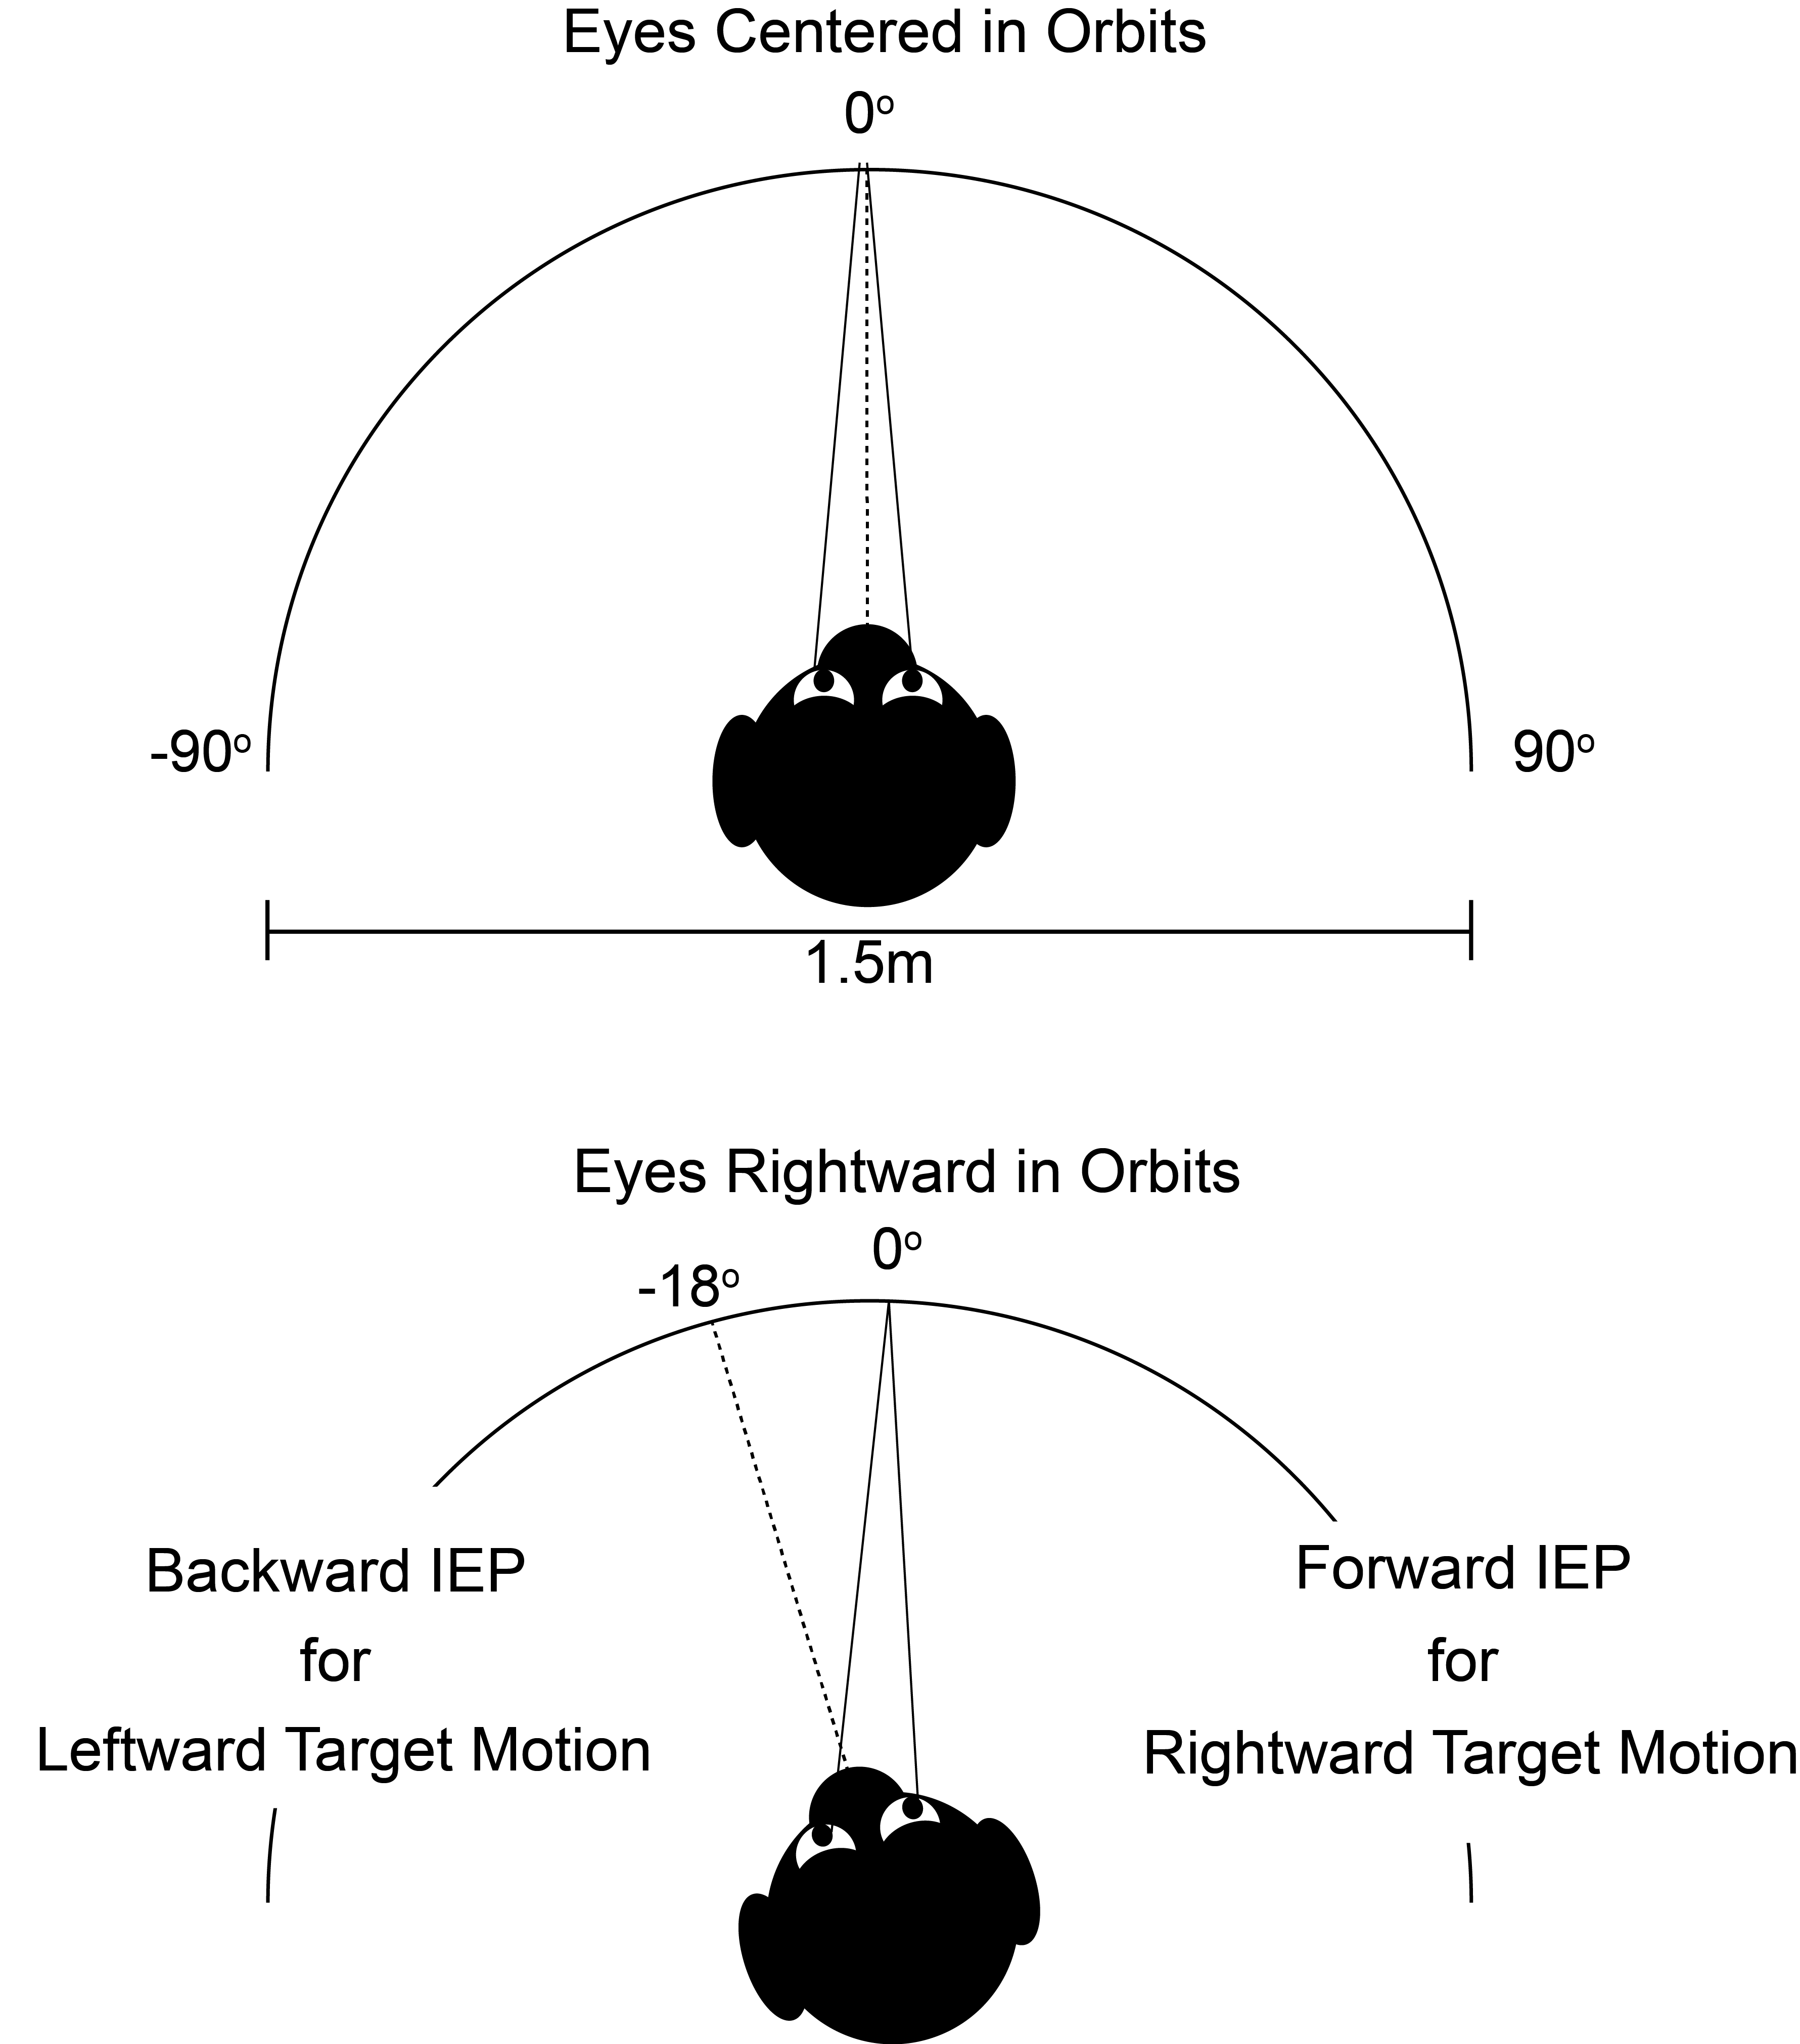
\includegraphics[width=0.7\linewidth]{./figs/IEPMethodsFigure}
\caption[Diagram of target presentation and initial eye position]{Diagram of Target Presentation and Initial Eye Position. This diagram shows the relative positions of the target presentation screen, a 1.5m hemisphere, and the subject seated at the center. We define zero degrees horizontal to be straight forward, aligned with the subject's midsagittal plane. We can present targets 90 deg in either direction. The top panel shows the eyes centered condition, where the eyes, gaze and head are all aligned with the same point on the screen. The bottom panel shows the the subject maintaining the eyes rightward in the orbits. This corresponds with the forward IEP condition for rightward movements, and the backward IEP condition for leftward movements.}
\label{fig:IEPMethodsFigure}
\end{figure}

\begin{figure}[h]
\centering
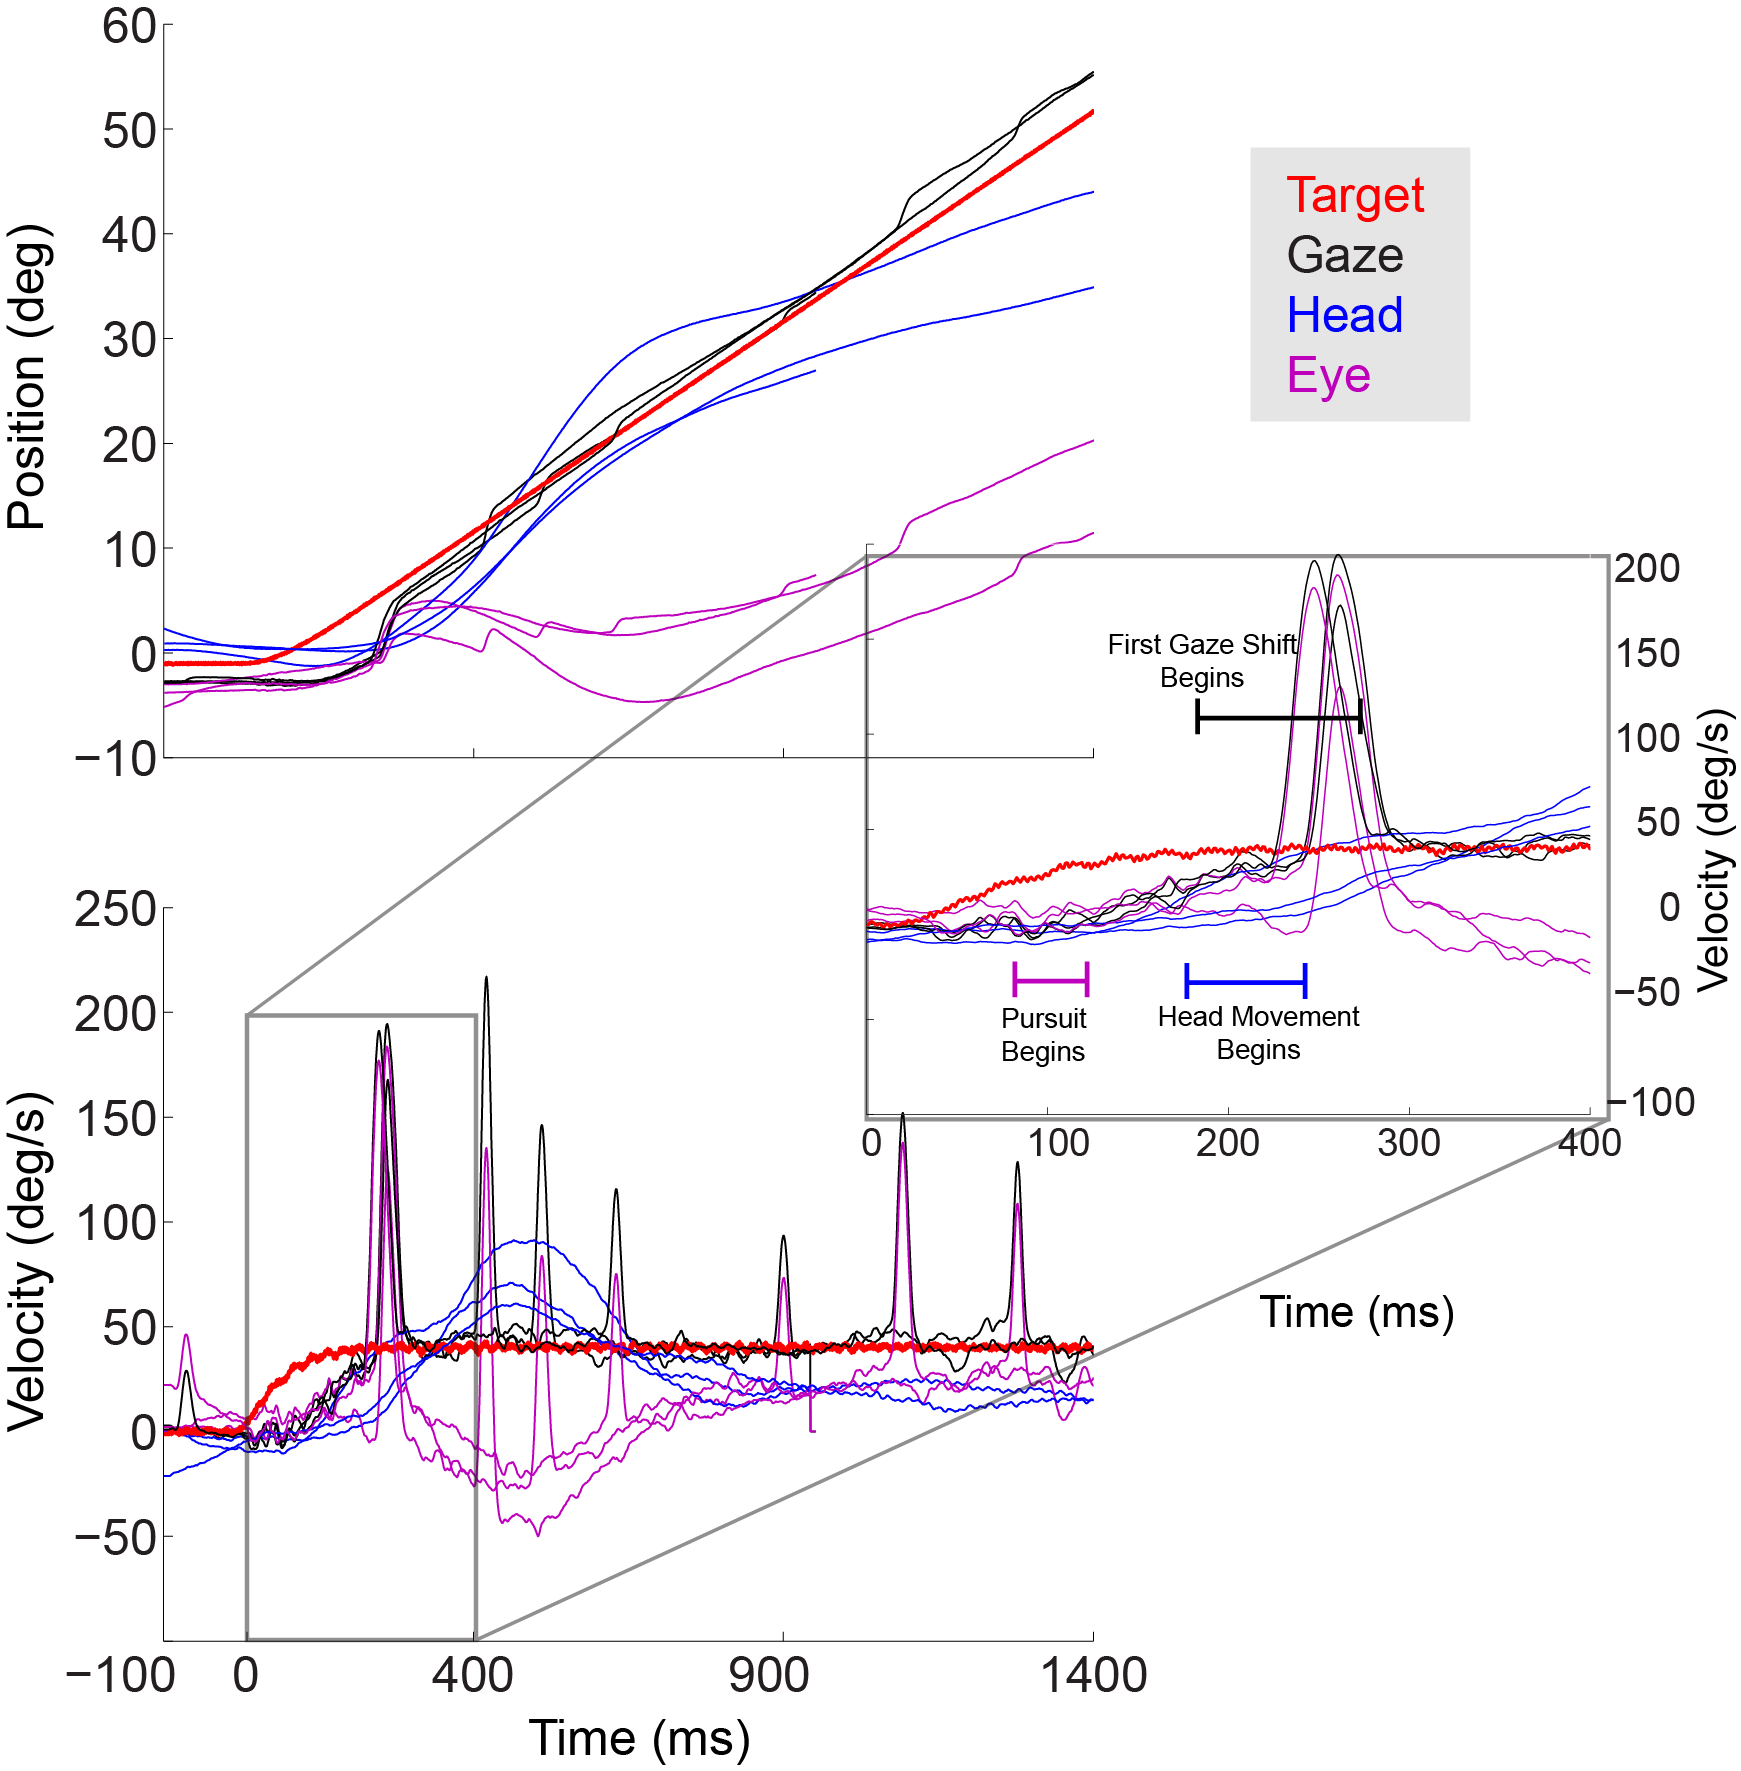
\includegraphics[width=0.7\linewidth]{./figs/CenterIEP}
\caption[Gaze Pursuit with Eyes Centered]{Centered IEP Condition. Example of subject's behavioral responses (gaze – black, head – blue, eye – purple) to visual targets moving at 30 deg/s (red) to the right when the eyes begin centered in the orbits. Horizontal bars indicate plus or minus one standard deviation of the latency of the different components of the movement (see Table 1).
}
\label{fig:CenterIEP}
\end{figure}


\begin{figure}[h]
\centering
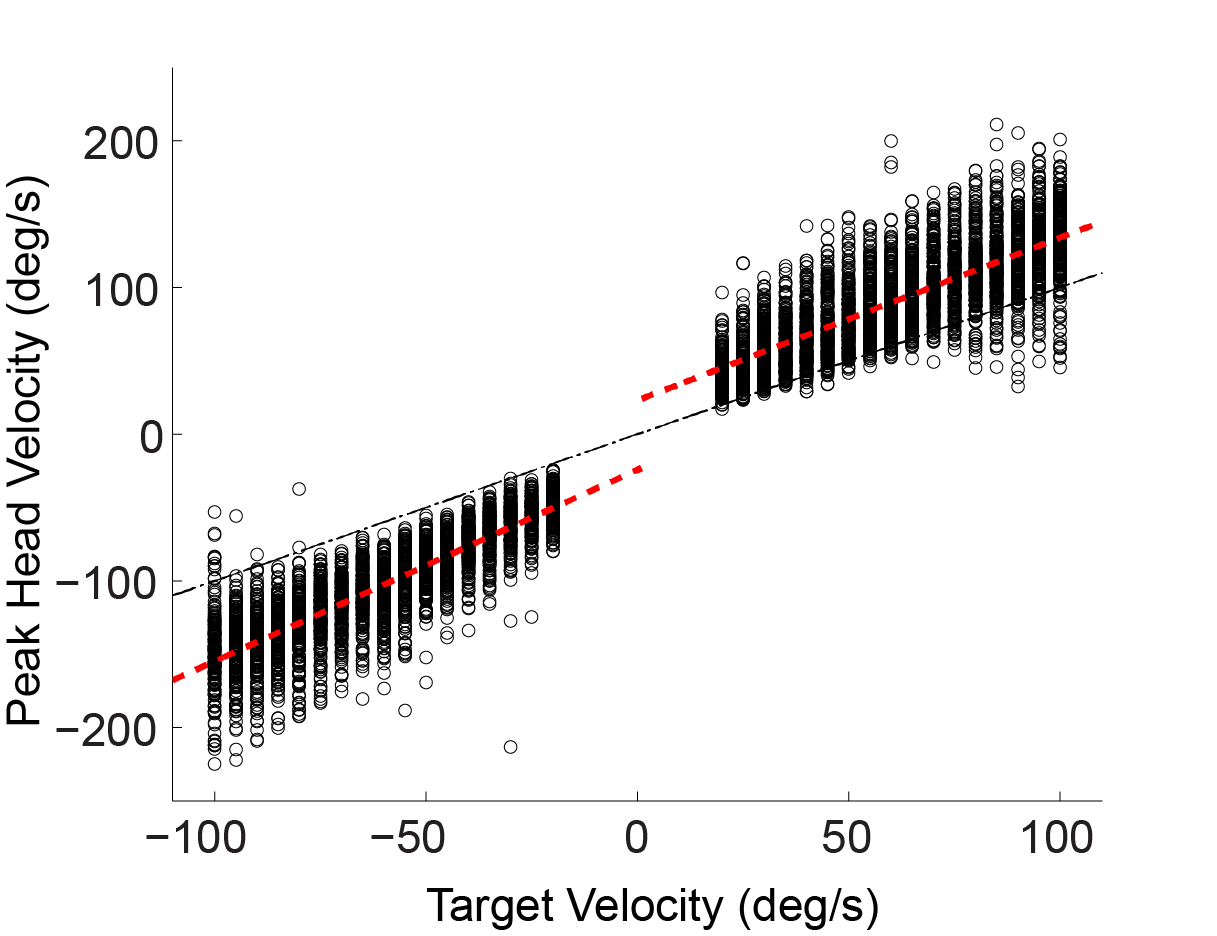
\includegraphics[width=0.7\linewidth]{./figs/CenterRegression}
\caption[Peak Head Velocity during Pursuit with Eyes Centered.]{Peak Head Velocity during Pursuit with Eyes Centered. The relationship between peak head velocity and target velocity. For each trial (n= 7412 from subject U) the peak velocity of the head during the first 500 ms of pursuit is plotted against the velocity of the target on that trial. Negative velocities indicate leftward motion. Unity line (Peak head velocity = Target Velocity) is shown (black dashed). Best linear fit polynomials are shown for each direction independently (red dashed).}
\label{fig:CenterRegression}
\end{figure}

\begin{table}[h]
\begin{tabular}{@{}lllccc@{}}
\toprule
Subject               & Direction                    & \multicolumn{1}{c}{IEP}          & \multicolumn{3}{l}{Latency (SD) in milliseconds movements}                                                         \\ \midrule
                      &                              &                                  & Pursuit                              & Gaze Shift                           & Head                                 \\
                      & \cellcolor[HTML]{EFEFEF}     & \cellcolor[HTML]{EFEFEF}Backward & \cellcolor[HTML]{EFEFEF}96.6 (20.6)  & \cellcolor[HTML]{EFEFEF}238.9 (54.0) & \cellcolor[HTML]{EFEFEF}246.6 (43.0) \\
                      & \cellcolor[HTML]{EFEFEF}Left & \cellcolor[HTML]{EFEFEF}Centered & \cellcolor[HTML]{EFEFEF}96.2 (20.0)  & \cellcolor[HTML]{EFEFEF}244.4 (56.1) & \cellcolor[HTML]{EFEFEF}254.4 (59.7) \\
\multicolumn{1}{c}{U} & \cellcolor[HTML]{EFEFEF}     & \cellcolor[HTML]{EFEFEF}Forward  & \cellcolor[HTML]{EFEFEF}95.9 (20.0)  & \cellcolor[HTML]{EFEFEF}254.4 (59.7) & \cellcolor[HTML]{EFEFEF}187.0 (21.2) \\
                      &                              & Backward                         & 93.7 (16.5)                          & 216.1 (48.9)                         & 257.5 (59.0)                         \\
                      & Right                        & Centered                         & 95.4 (18.1)                          & 238.9 (52.3)                         & 224.2 (34.0)                         \\
                      &                              & Forward                          & 95.5 (18.5)                          & 253.7 (58.5)                         & 200.7 (25.5)                         \\
                      & \cellcolor[HTML]{EFEFEF}     & \cellcolor[HTML]{EFEFEF}Backward & \cellcolor[HTML]{EFEFEF}103.8 (21.7) & \cellcolor[HTML]{EFEFEF}202.9 (43.7) & \cellcolor[HTML]{EFEFEF}247.6 (52.1) \\
                      & \cellcolor[HTML]{EFEFEF}Left & \cellcolor[HTML]{EFEFEF}Centered & \cellcolor[HTML]{EFEFEF}105.8 (22.8) & \cellcolor[HTML]{EFEFEF}211.4 (44.0) & \cellcolor[HTML]{EFEFEF}220.2 (38.9) \\
\multicolumn{1}{c}{S} & \cellcolor[HTML]{EFEFEF}     & \cellcolor[HTML]{EFEFEF}Forward  & \cellcolor[HTML]{EFEFEF}105.5 (22.5) & \cellcolor[HTML]{EFEFEF}220.2 (39.9) & \cellcolor[HTML]{EFEFEF}204.6 (31.4) \\
                      &                              & Backward                         & 100.9 (19.7)                         & 212.2 (41.4)                         & 215.5 (41.7)                         \\
                      & Right                        & Centered                         & 101.5 (20.1)                         & 228.1 (44.9)                         & 210.3 (33.2)                         \\
                      &                              & Forward                          & 100.7 (19.6)                         & 251.8 (51.2)                         & 204.7 (27.8)                         \\ \bottomrule
\end{tabular}
\caption[Latency]{The mean and standard deviation (in parentheses) of the latency of pursuit initiation the first gaze shift and head movement initiation for the two subjects in milliseconds after the target begins to move. Each direction is calculated independently. Note that backward IEP and forward IEP are relative to the direction of target motion (Fig~\ref{fig:IEPMethodsFigure}).  Trials in which no head movements or gaze shifts are made within the first 400ms are not included in the average latency.}
\label{tab:Ramp}
\end{table}

\begin{figure}[h]
\centering
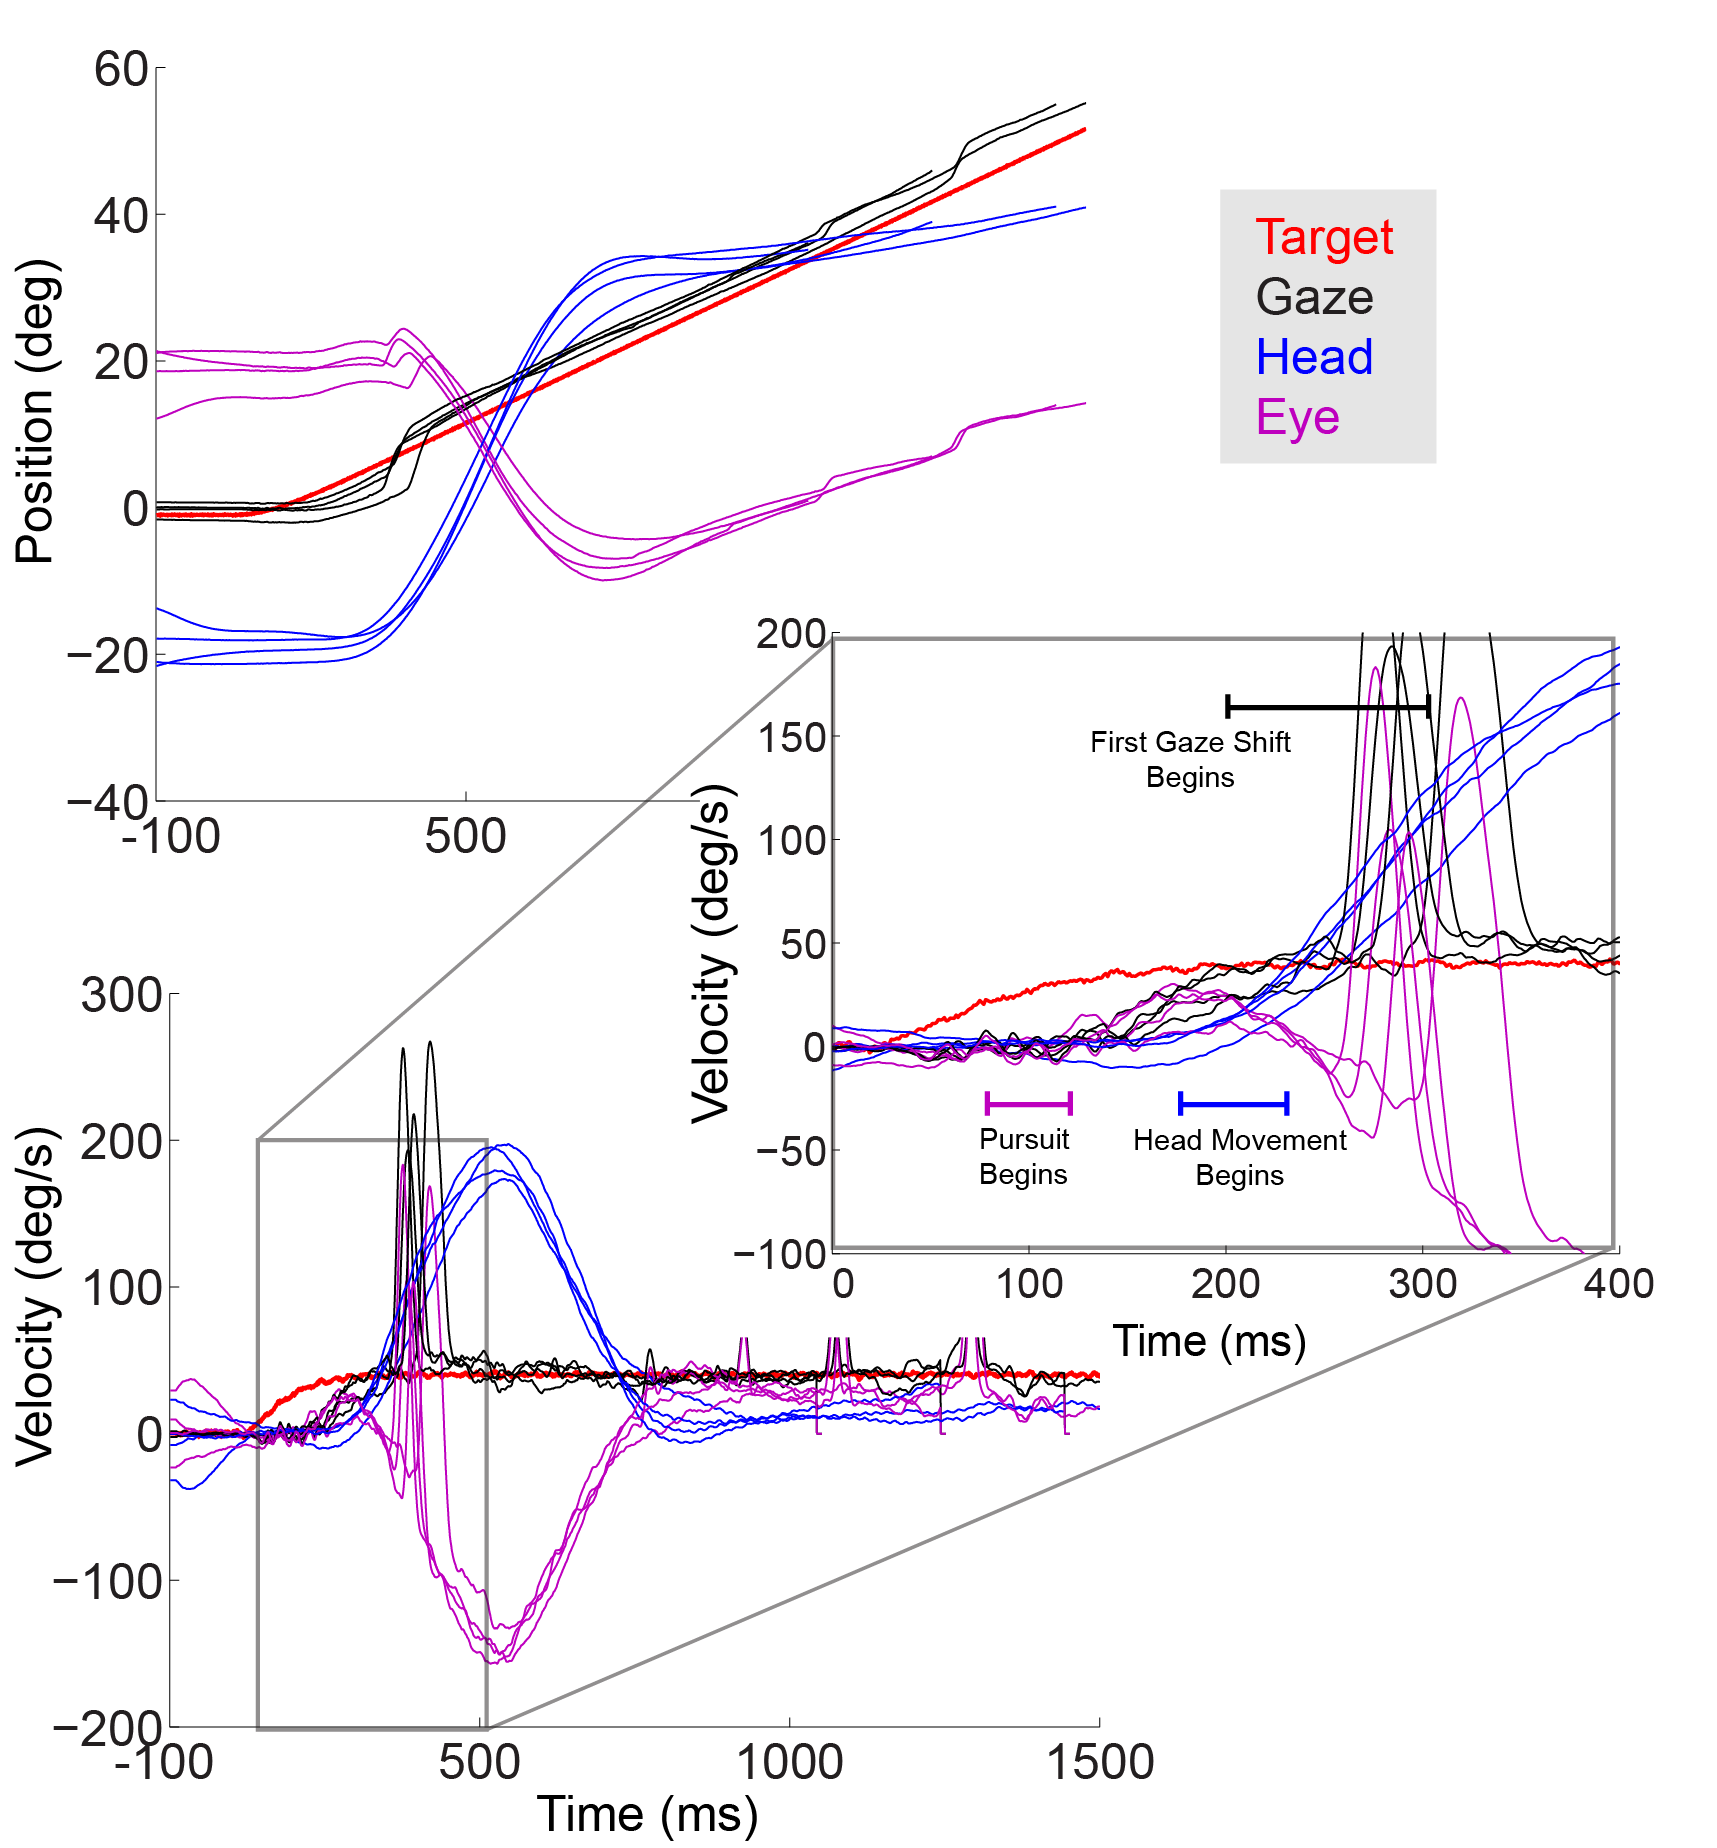
\includegraphics[width=0.7\linewidth]{./figs/ForwardIEP}
\caption[Behavior during Forward IEP]{Forward IEP Condition. Example of subject's behavioral responses (gaze – black, head – blue, eye – purple) to visual targets moving at 30 deg/s (red) to the right when the eyes begin forward in the orbits. Horizontal bars indicate plus or minus one standard deviation of the latency of the different components of the movement (see Table 1).
}
\label{fig:ForwardIEP}
\end{figure}

\begin{figure}[h]
\centering
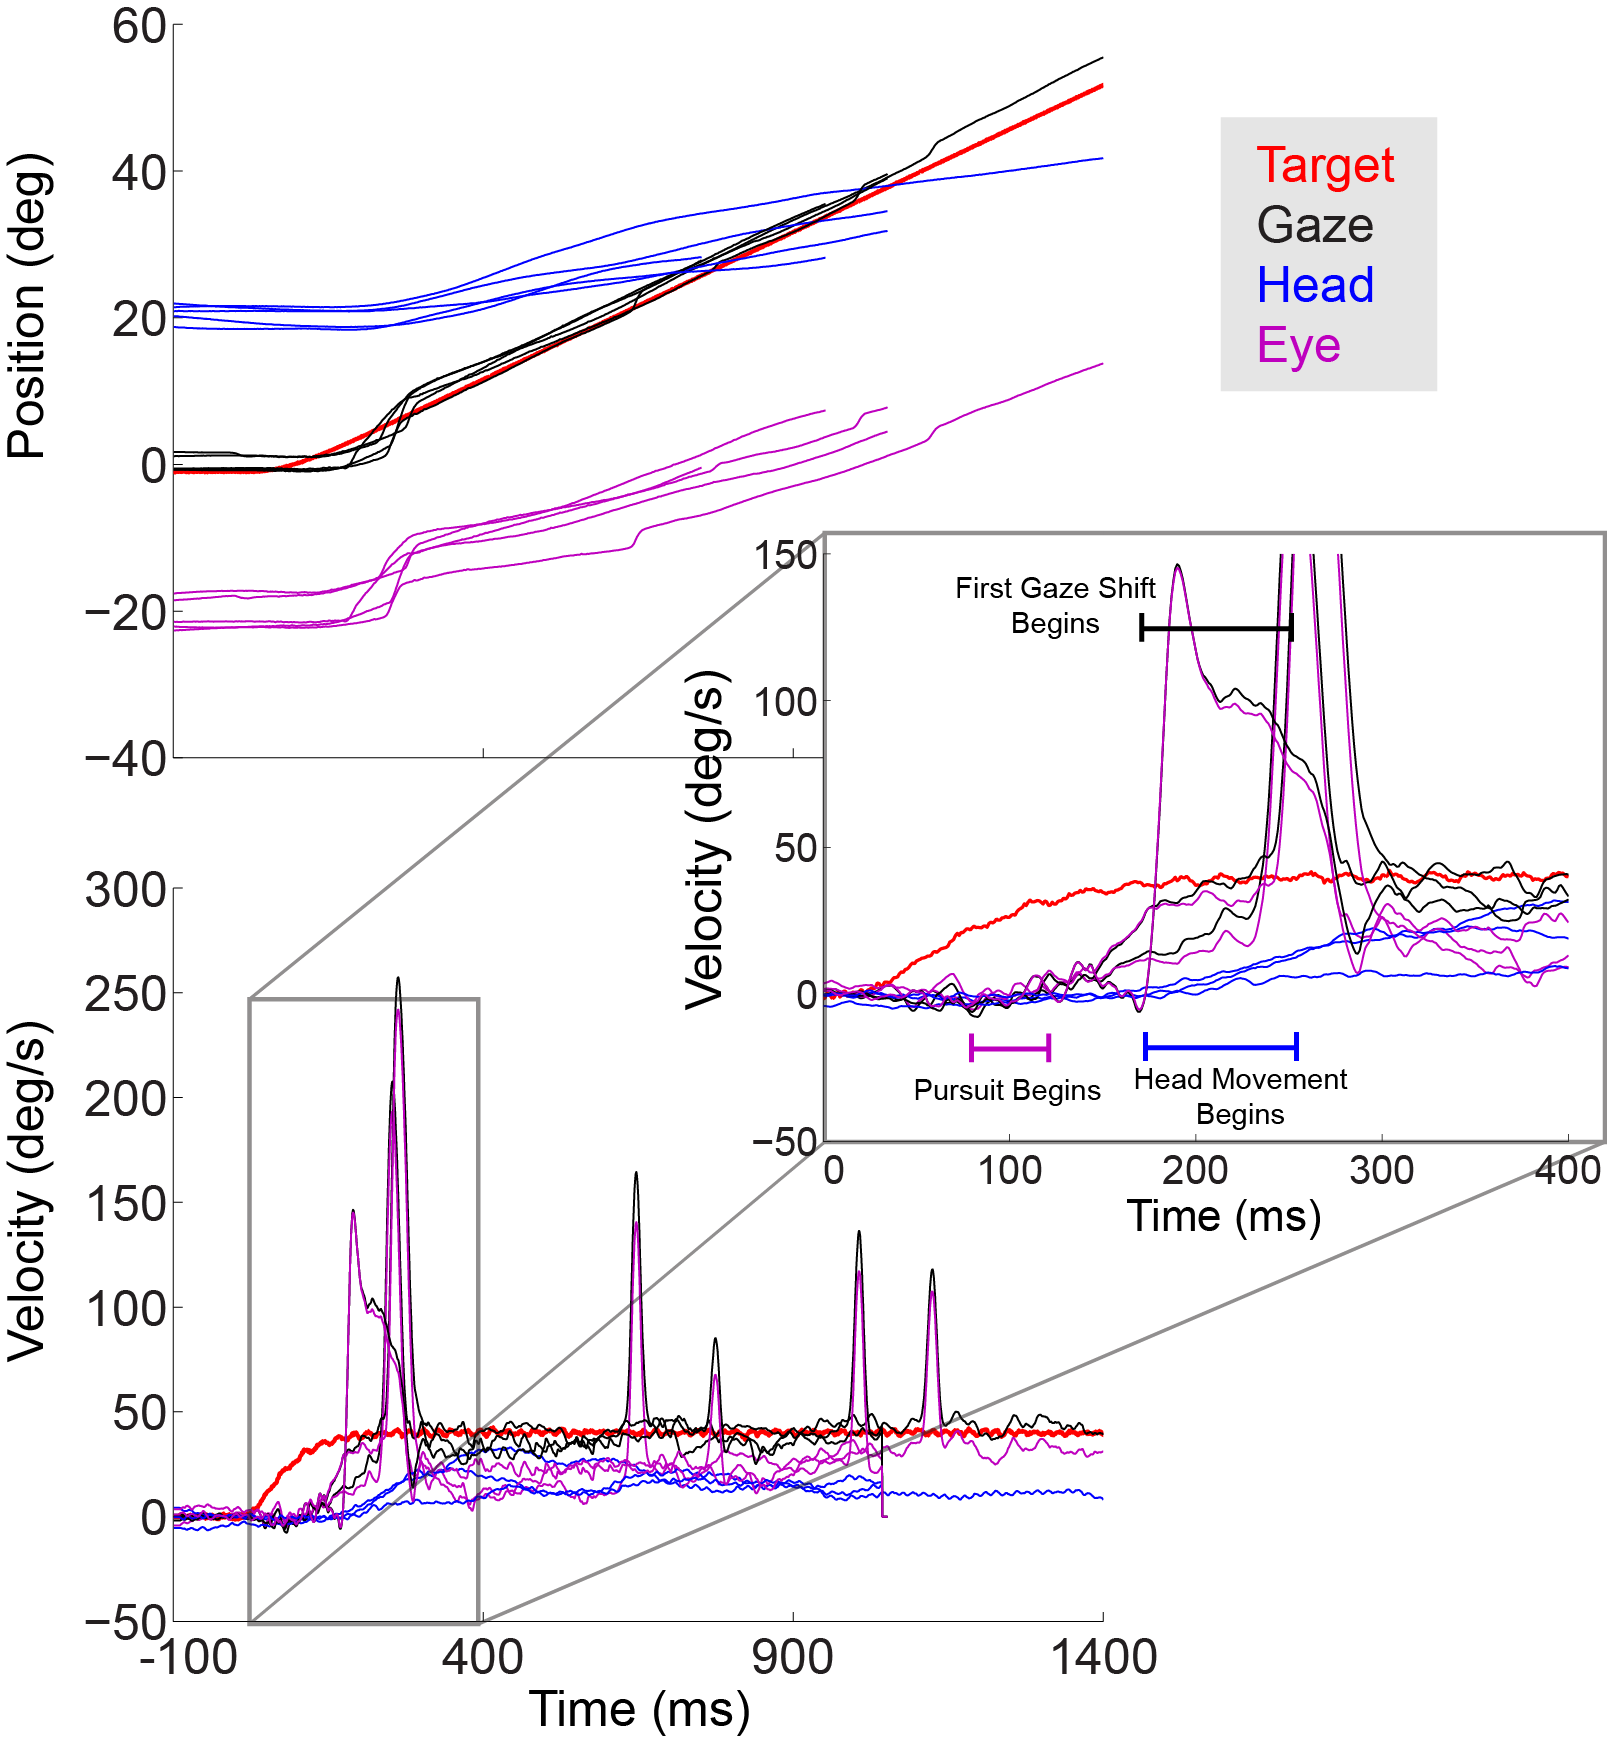
\includegraphics[width=0.7\linewidth]{./figs/BackwardIEP}
\caption[Behavior with forward IEP]{Backward IEP Condition. Example of subject's behavioral responses (gaze – black, head – blue, eye – purple) to visual targets moving at 30 deg/s (red) to the right when the eyes begin forward in the orbits. Horizontal bars indicate plus or minus one standard deviation of the latency of the different components of the movement (see Table 1).}
\label{fig:BackwardIEP}
\end{figure}

\begin{figure}
\centering
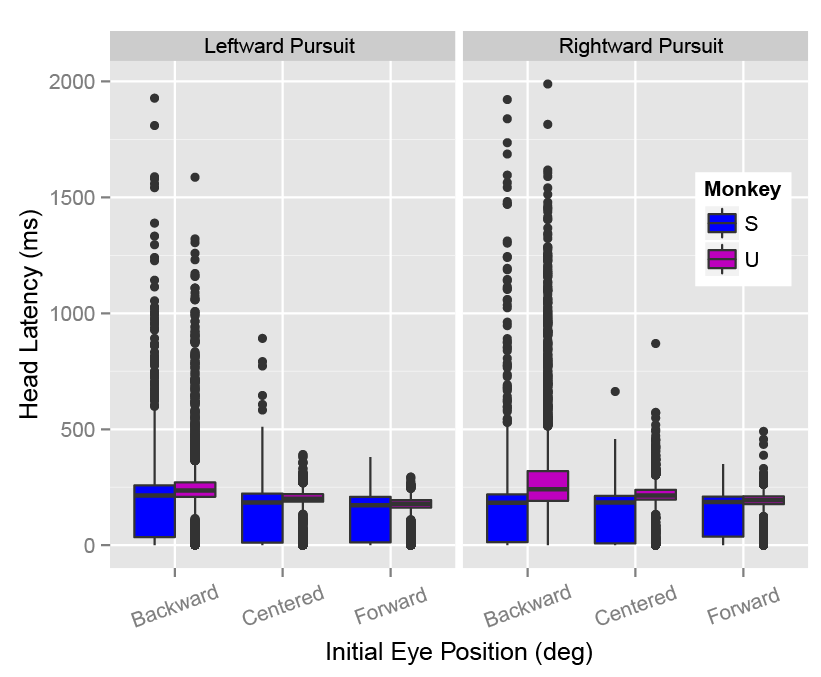
\includegraphics[width=0.7\linewidth]{./figs/RampHeadLatency}
\caption[Head latency during ramp trials]{Head Latency during Gaze Pursuit. The effect of initial eye position on the latency of head movements during leftward (left panel) and rightward (right panel) gaze pursuit made in response to position ramp target motion. Responses from two subjects, S (blue) and U (purple) are shown.}
\label{fig:RampHeadLatency}
\end{figure}

\begin{figure}[h]
\centering
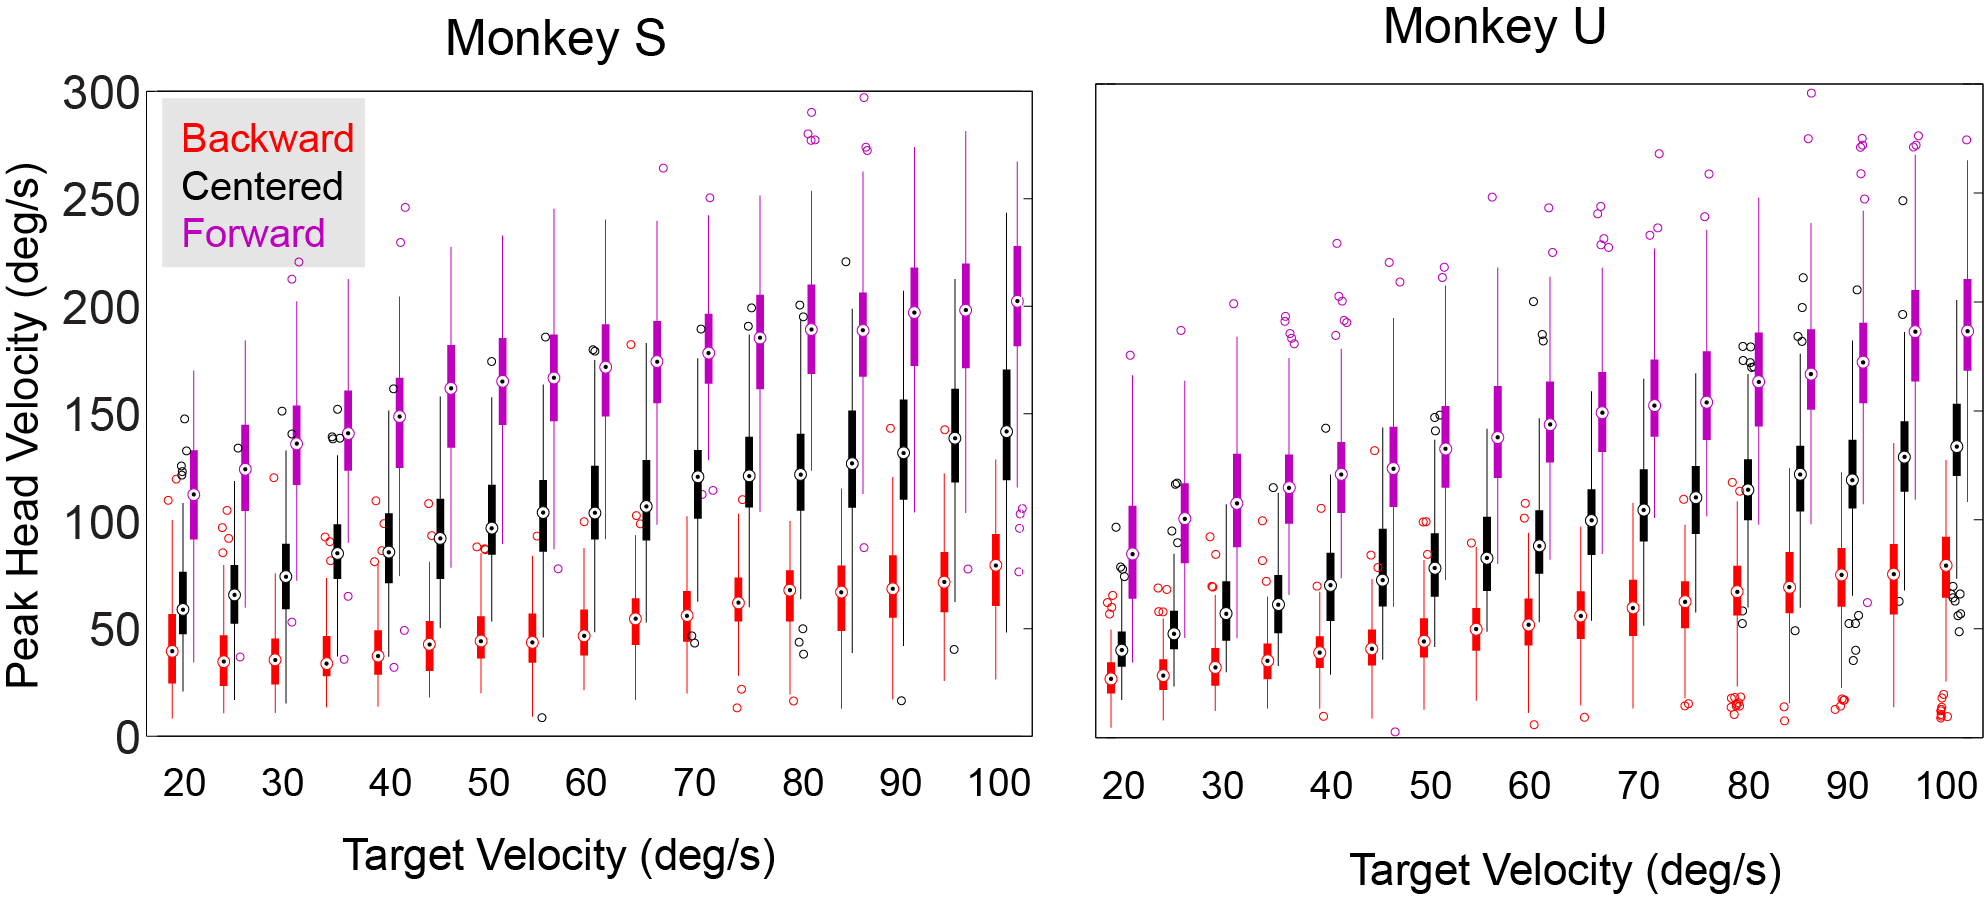
\includegraphics[width=0.9\linewidth]{./figs/RampBoxplot}
\caption[Peak Head Velocity during Pursuit of Ramp Targets]{Comparison of Peak Head Velocity during Pursuit with Different Initial Eye Positions. Box plots indicating the median (center) and 25th – 75th percentile (box) for the three IEP conditions at each of the rightward target velocities tested (20 -100 deg/s in 5 deg increments). Whiskers extend 1.5 times the length of the box and individual trials not within this interval are plotted individually.}
\label{fig:RampBoxplot}
\end{figure}

\begin{figure}
\centering
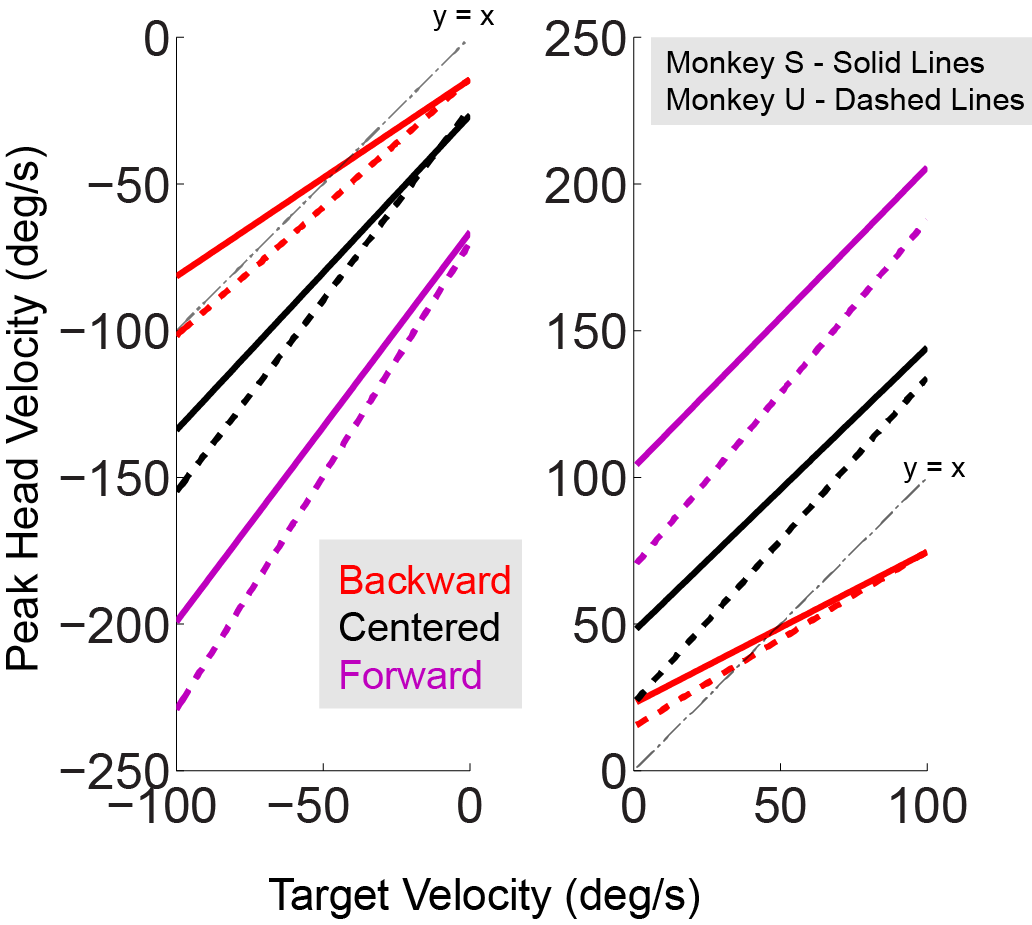
\includegraphics[width=0.7\linewidth]{./figs/RampRegressions}
\caption{Comparison of Linear Fit Relationships between Target and Peak Head Velocities for Pursuit with Different Initial Eye Positions and Subjects. Linear fit regression model for the relationship between target velocity and peak head velocity. Leftward and rightward movements are fit independently. Colors indicate the IEP condition (red – Backward IEP, black- Centered IEP, purple – Forward IEP). Fits from subject S are shown as solid lines and fits from subject U are shown in dashed lines. The unity line (Target Velocity = Peak head velocity) is shown (gray dashed).}
\label{fig:RampRegressions}
\end{figure}

\begin{figure}
\centering
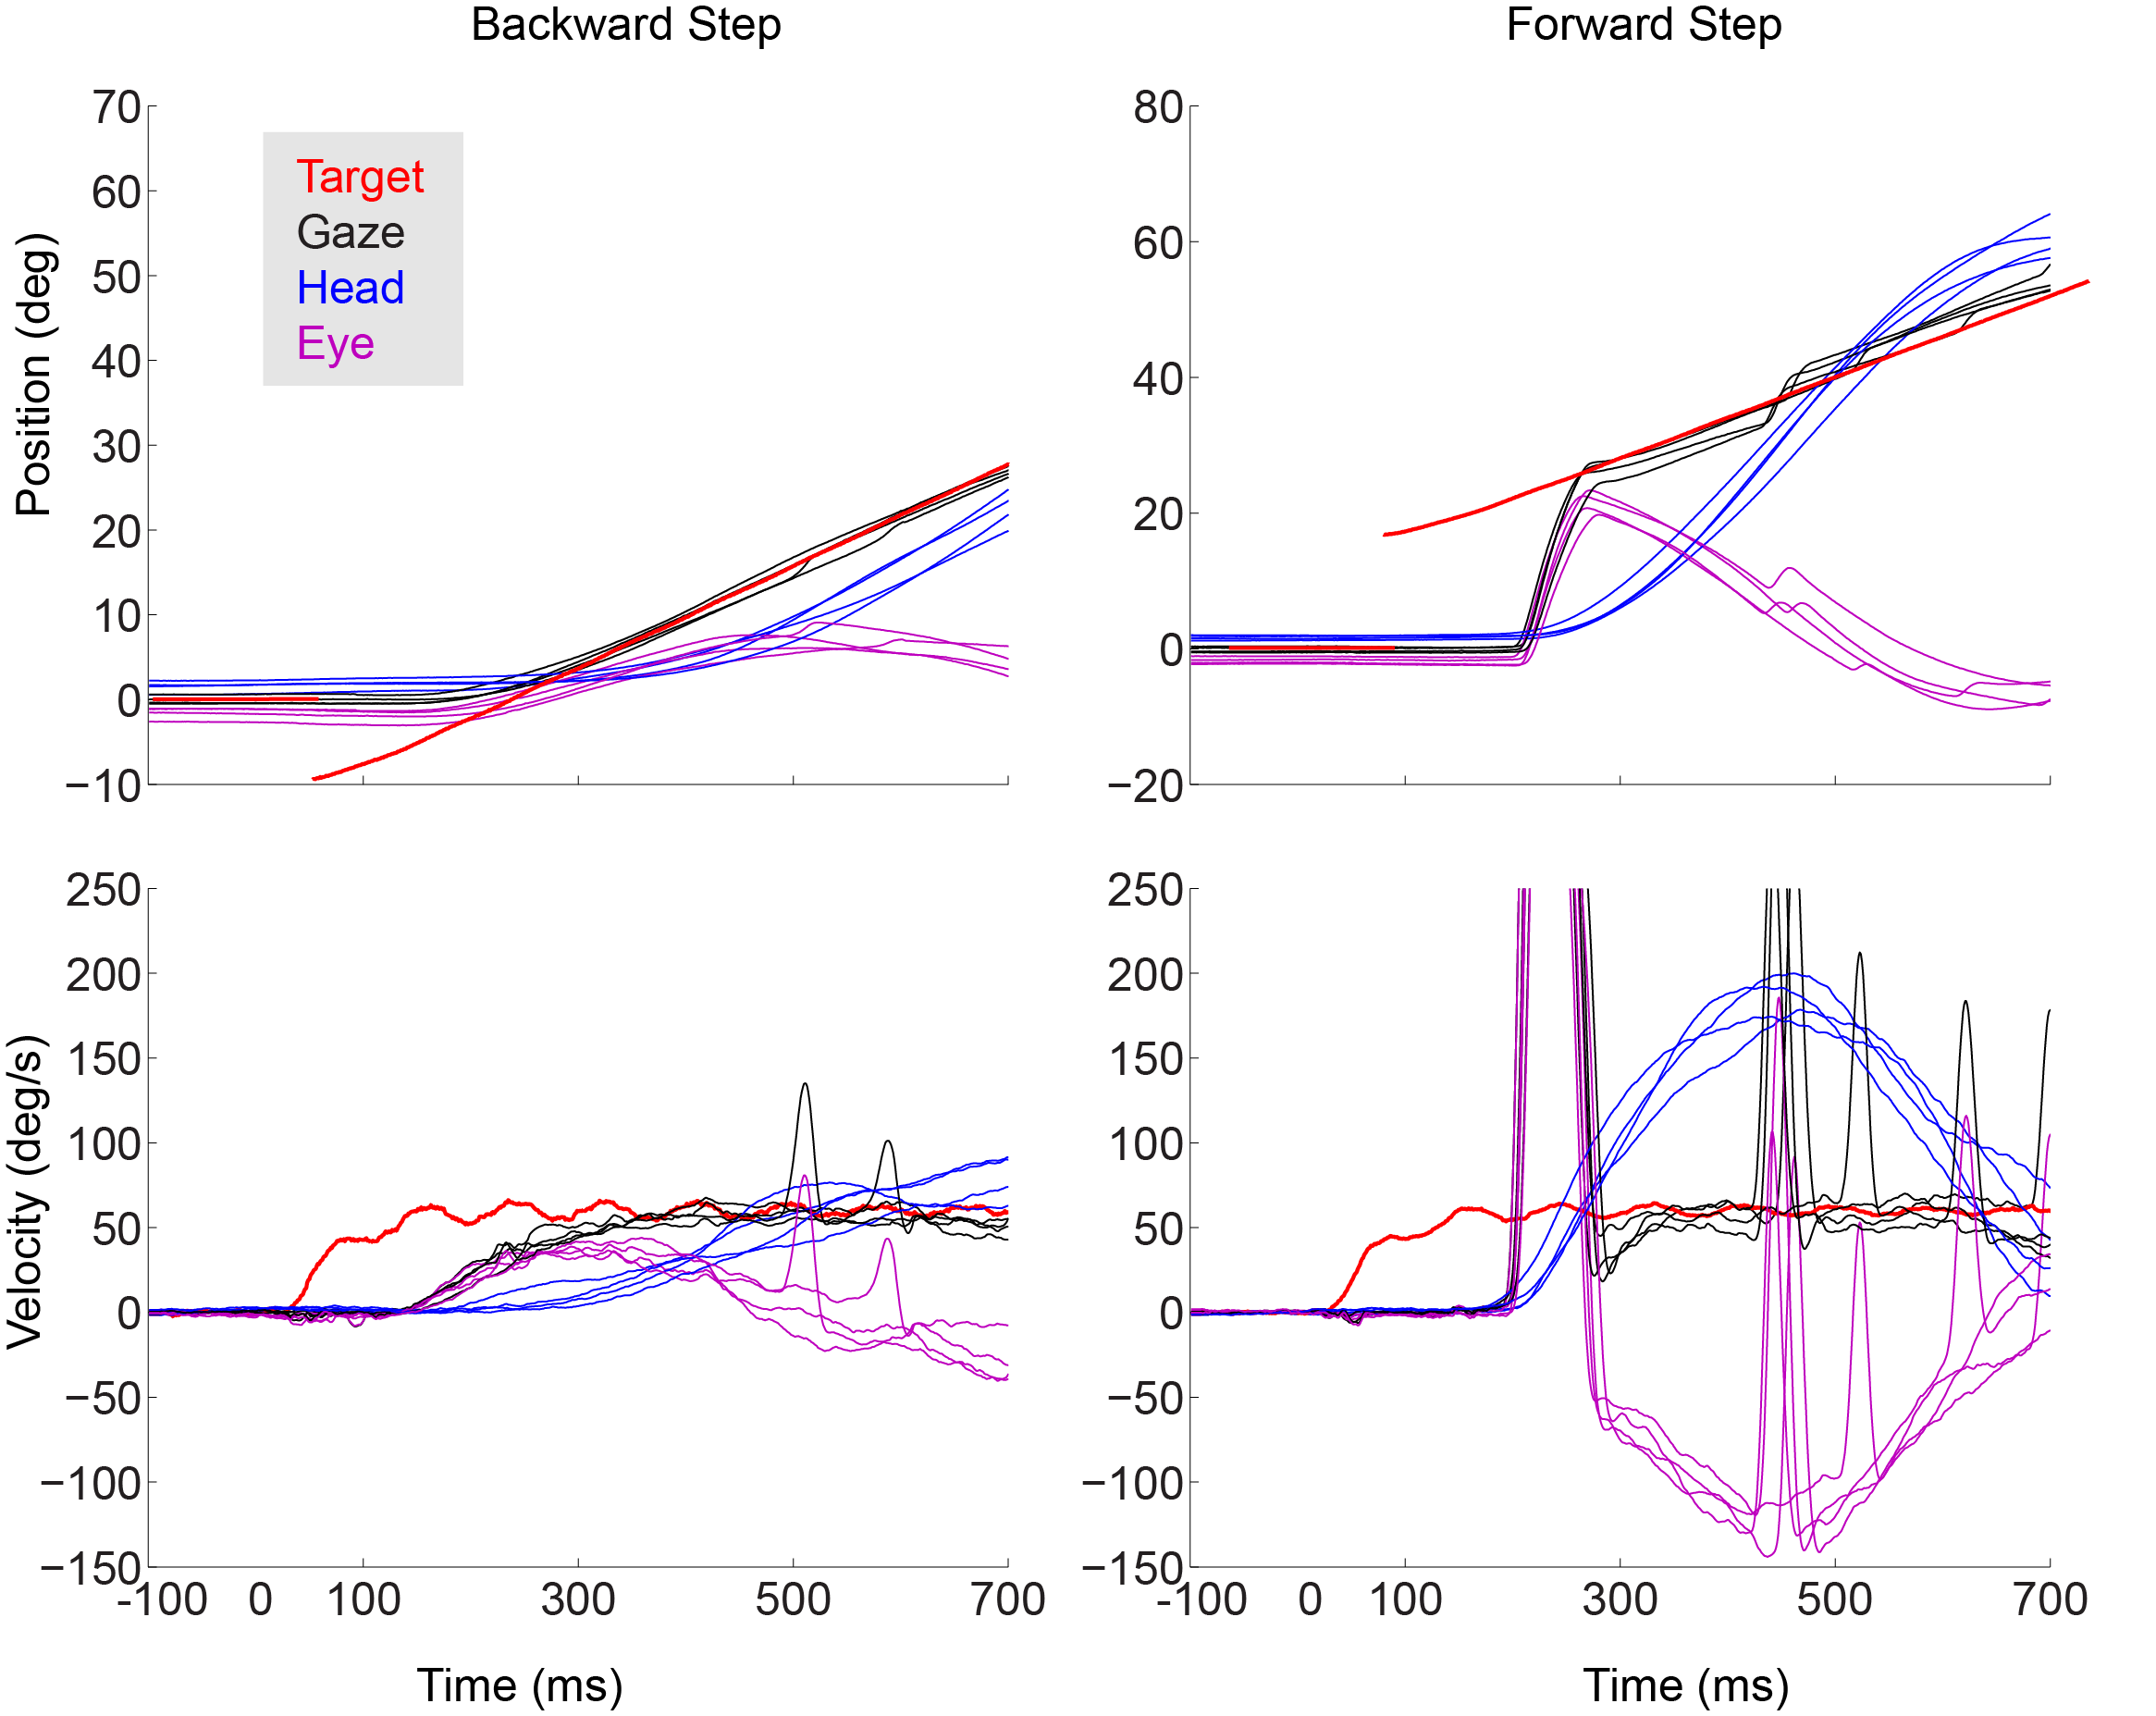
\includegraphics[width=0.9\linewidth]{./figs/StepRampExample}
\caption[Step-Ramp Behavior]{Gaze Pursuit of Forward and Backward Step-Ramp Stimuli. Example of subject's behavioral responses (gaze – black, head – blue, eye – purple) to visual targets moving at 60 deg/s (red) to the right when the target steps backward (left) or forward (right) just prior to target motion.}
\label{fig:StepRampExample}
\end{figure}

\begin{figure}
\centering
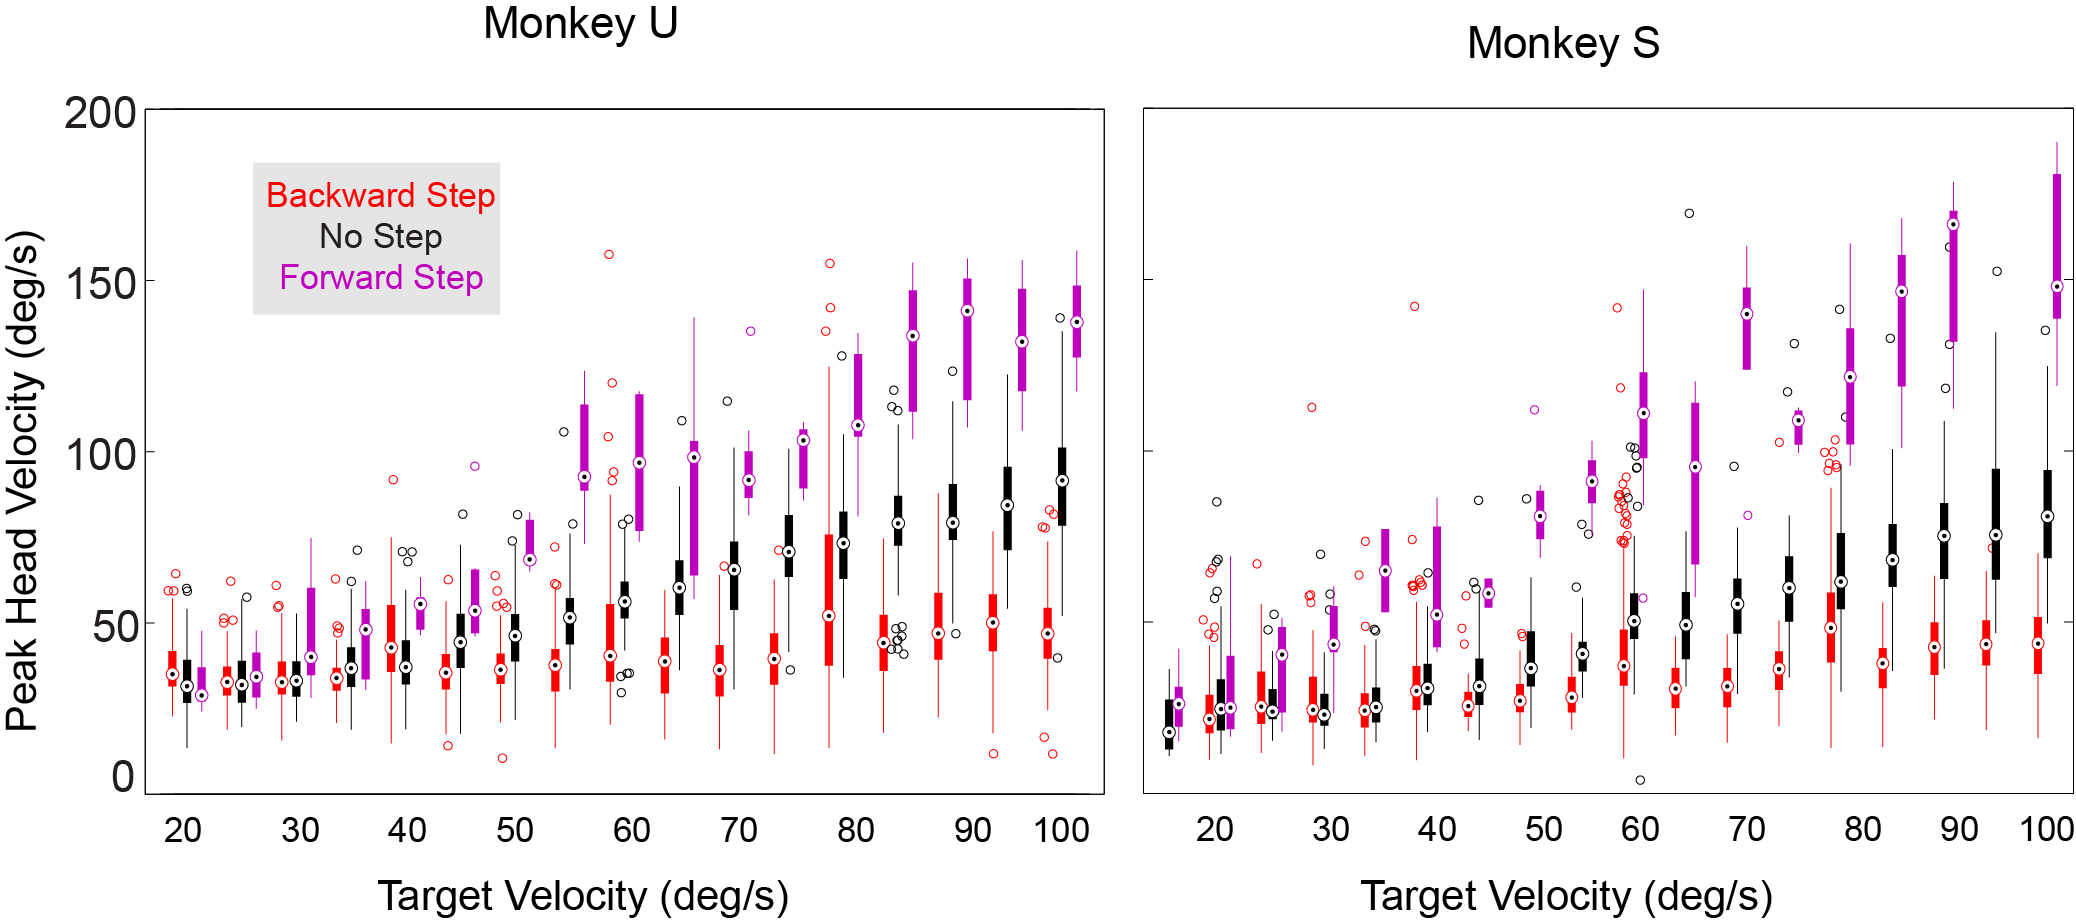
\includegraphics[width=0.9\linewidth]{./figs/StepRampBoxplot}
\caption[Step-Ramp Peak Head Velocity]{Comparison of Peak Head Velocities during Pursuit of Step-Ramp Stimuli of Different Step Sizes. Box plots indicating the median (center) and 25th – 75th percentile (box) for the three step-ramp conditions at each of the rightward target velocities tested (20 -100 deg/s in 5 deg increments. Also 10 deg/s movements from subject S). Whiskers extend 1.5 times the length of the box and individual trials not within this interval are plotted individually.}
\label{fig:StepRampBoxplot}
\end{figure}

\begin{figure}
\centering
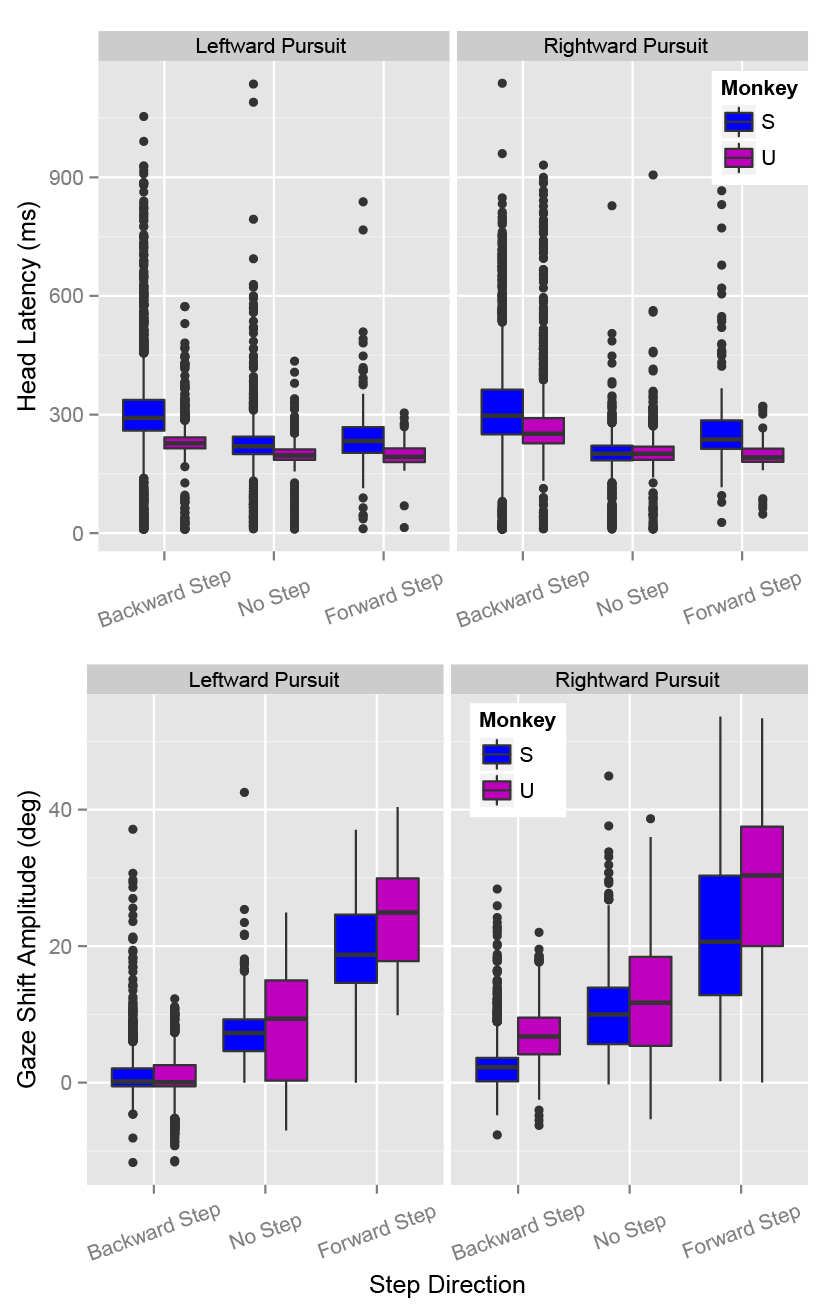
\includegraphics[width=0.7\linewidth]{./figs/StepRampLatencyandGSAmp}
\caption[Head Latency and Gaze Shift Amplitude during Step Ramp Trials]{Head Latency and Gaze Shift Amplitude during Step Ramp Trials. The latency of head movements and the amplitude of the first gaze shift during step ramp trials for monkeys S (blue) and U (purple). Top: The effect of step direcion on head latency during leftward (left panel) and rightward (right panel) pursuit. Bottom: The effect of step direction on the amplitude of the first gaze shift during pursuit. Negative amplitude represents gaze shifts in the opposite direction of target motion.}
\label{fig:StepRampLatencyandGSAmp}
\end{figure}

\begin{figure}
\centering
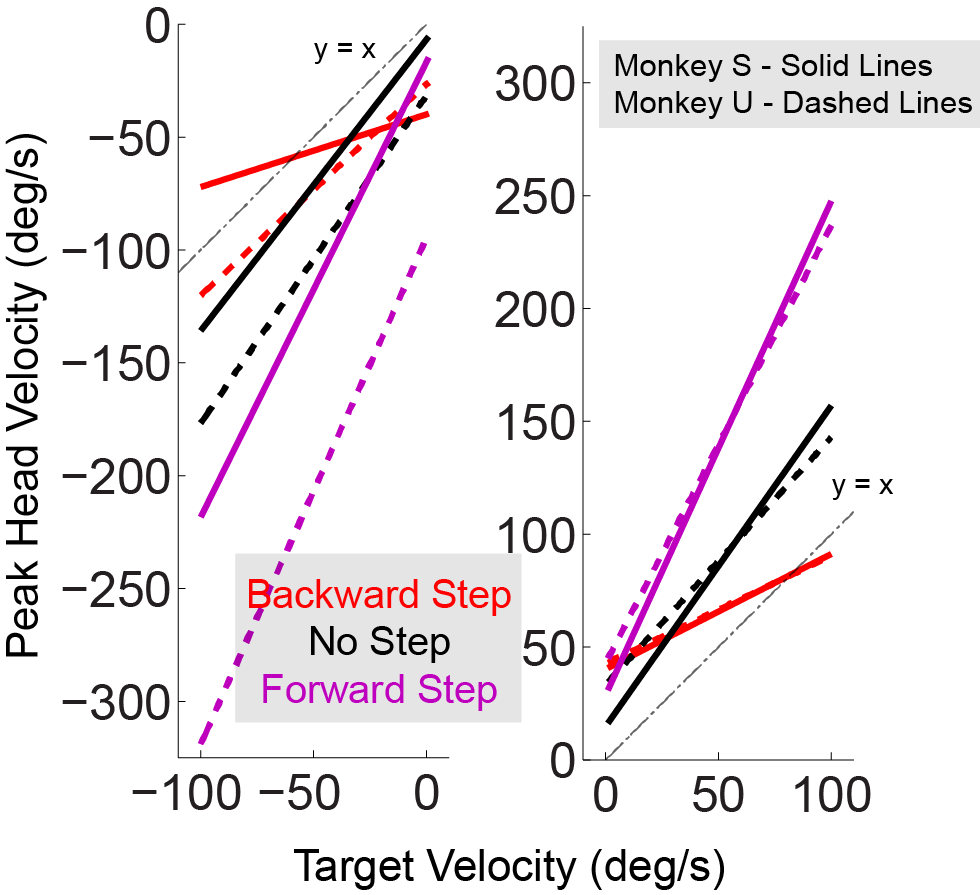
\includegraphics[width=0.9\linewidth]{./figs/StepRampRegressions}
\caption{Comparison of Linear Fit Relationships between Target and Peak Head Velocities for Pursuit of Step-Ramp Stimuli with different Step Sizes and Subjects. Linear fit regression model for the relationship between target velocity and peak head velocity. Leftward and rightward movements are fit independently. Values shown in table 4. Colors indicate the step-ramp condition (red – Backward Step, black-No Step, purple – Forward Step). Fits from subject S are shown as solid lines and fits from subject U are shown in dashed lines. The unity line (Target Velocity = Peak head velocity) is shown (gray dashed).}
\label{fig:StepRampRegressions}
\end{figure}

\begin{table}[h]
\centering
\resizebox{\textwidth}{!}{%
\begin{tabular}{@{}ccccccr@{}}
\toprule
Subject & Direction                    & Step                             & \multicolumn{3}{c}{Latency (SD) in milliseconds}                                                                   &                                                                                     \\ \cmidrule(r){1-6}
        &                              &                                  & Pursuit                              & Gaze Shift                           & Head                                 & \multirow{-2}{*}{\begin{tabular}[c]{@{}c@{}}Gaze Shift\\  in deg (SD)\end{tabular}} \\ \cmidrule(l){7-7} 
        & \cellcolor[HTML]{EFEFEF}     & \cellcolor[HTML]{EFEFEF}Backward & \cellcolor[HTML]{EFEFEF}98.1 (23.5)  & \cellcolor[HTML]{EFEFEF}221.4 (71.8) & \cellcolor[HTML]{EFEFEF}230.8 (26.5) & \cellcolor[HTML]{EFEFEF}1.4 (3.2)                                                   \\
        & \cellcolor[HTML]{EFEFEF}Left & \cellcolor[HTML]{EFEFEF}No Step  & \cellcolor[HTML]{EFEFEF}94.4 (19.6)  & \cellcolor[HTML]{EFEFEF}251.8 (59.5) & \cellcolor[HTML]{EFEFEF}201.2 (25.2) & \cellcolor[HTML]{EFEFEF}-9.8 (6.8)                                                  \\
U       & \cellcolor[HTML]{EFEFEF}     & \cellcolor[HTML]{EFEFEF}Forward  & \cellcolor[HTML]{EFEFEF}121.1 (38.3) & \cellcolor[HTML]{EFEFEF}242.9 (30.4) & \cellcolor[HTML]{EFEFEF}202.3 (29.6) & \cellcolor[HTML]{EFEFEF}-24.6 (7.9)                                                 \\
        &                              & Backward                         & 97.8 (24.2)                          & 316.2 (85.5)                         & 257.2 (44.5)                         & 6.2 (5.1)                                                                           \\
        & Right                        & No Step                          & 91.4 (14.8)                          & 238.1 (52.9)                         & 206.8 (31.3)                         & 12.7 (8.0)                                                                          \\
        &                              & Forward                          & 113.8 (30.8)                         & 217.2 (31.3)                         & 201.8 (31.8)                         & 29.6 (11.3)                                                                         \\
        & \cellcolor[HTML]{EFEFEF}     & \cellcolor[HTML]{EFEFEF}Backward & \cellcolor[HTML]{EFEFEF}115.2 (27.1) & \cellcolor[HTML]{EFEFEF}248.8 (61.2) & \cellcolor[HTML]{EFEFEF}289.1 (47.3) & \cellcolor[HTML]{EFEFEF}0.0 (3.4)                                                   \\
        & \cellcolor[HTML]{EFEFEF}Left & \cellcolor[HTML]{EFEFEF}No Step  & \cellcolor[HTML]{EFEFEF}109.2 (21.7) & \cellcolor[HTML]{EFEFEF}217.4 (38.3) & \cellcolor[HTML]{EFEFEF}227.2 (39.9) & \cellcolor[HTML]{EFEFEF}-7.4 (3.5)                                                  \\
S       & \cellcolor[HTML]{EFEFEF}     & \cellcolor[HTML]{EFEFEF}Forward  & \cellcolor[HTML]{EFEFEF}141.9 (41.1) & \cellcolor[HTML]{EFEFEF}208.2 (32.0) & \cellcolor[HTML]{EFEFEF}237.8 (46.7) & \cellcolor[HTML]{EFEFEF}-18.9 (8.9)                                                 \\
        &                              & Backward                         & 114.7 (26.9)                         & 261.9 (69.5)                         & 286.1 (53.1)                         & 0.9 (2.8)                                                                           \\
        & Right                        & No Step                          & 106.9 (24.3)                         & 218.3 (26.3)                         & 207.2 (34.2)                         & 10.5 (6.0)                                                                          \\
        &                              & Forward                          & 142.0 (47.0)                         & 229.1 (33.6)                         & 236.8 (41.9)                         & 21.8 (12.6)                                                                         \\ \bottomrule
\end{tabular}
}
\caption[Latency during Step Ramp]{The mean and standard deviation (in parentheses) of the latency of pursuit initiation, the first gaze shift, and head movement initiation as well as the amplitude of the first gaze shift (if one is observed in the first 400ms) for the two subjects made during each of the step-ramp conditions. Each direction is calculated independently. Trials in which no head movements or gaze shifts are made within the first 400ms are not included in the average latency.}
\label{tab:StepRamp}
\end{table}

\section{Results}
\subsection{Controlling Initial Eye Position}
We recorded 37,476 trials (14,790 from monkey S; 22,686 from U) in which subjects successfully completed all requirements described in the methods for task 1. At the start of each trial, subjects aligned their heads in one of three orientations relative to the fixation target, resulting in three different initial positions of the eyes in the orbits. First, we will describe the behavior when the eyes begin centered in the orbits, which is likely to be the assumed normal behavior in experiments that do not control initial eye position. Despite variability and idiosyncratic behavior between subjects, as well as slight differences between movements to the left and right, we can discuss the relative timing of the gaze, eye and head movements that we observed.

In figure~\ref{fig:CenterIEP}, we present the positions and velocities of the eyes, head and gaze as a subject pursues a visual target that accelerates to and maintains a speed of 40 deg/s. This figure and the values described here describe the behavior of monkey S. Data from monkey U are similar and can be found in table ~\ref{tab:Ramp}. In the trials presented here, the eyes are centered in the orbits at the beginning of the trial. This means that the head and gaze are both pointed directly at the target, which appears at 0 degrees horizontally in our coordinate system (see fig~\ref{fig:IEPMethodsFigure}). We align a head-mounted laser with the mid-sagittal plane of the subjects and consider the head to be aligned with the target when the head-mounted laser overlaps with the target laser. We show 100ms of fixation before the target (red line) begins to move. Approximately 100 ms later, the eyes (purple lines) and gaze (black lines) begin to accelerate. The horizontal purple bar on the inset panel represents plus or minus one standard deviation from the mean pursuit latency from this subject. The acceleration of smooth pursuit is interrupted by a gaze shift, visible as a rapid acceleration and deceleration of the eyes. This corrects for the position error that accumulates during the latency period before smooth pursuit begins. The amount of position error that accumulates increases with faster target velocities meaning the amplitude of this gaze shift is dependent on the velocity of the target. The horizontal black bar indicates plus or minus one standard deviation from the mean time of the first gaze shift during pursuit. 

About the same time as the gaze shift is initiated, the head (blue) also begins to move in the direction of target motion. The horizontal blue bar in Figure~\ref{fig:CenterIEP}(inset) extends one standard deviation from the mean time of head movement onset. In the examples shown here, the head continues to accelerate, exceeding the velocity of the target. The variability of the peak head velocity is quite large, and will be described in more detail in Figure~\ref{fig:CenterRegression}. During this head movement, gaze pursuit velocity is relatively stable, proportional to the velocity of the target, though occasionally interrupted by gaze shifts. To facilitate this, the eyes decelerate, and begin to rotate in the orbits in the opposite direction of target motion at the appropriate speed to maintain a constant gaze pursuit velocity.  

In Figure~\ref{fig:CenterRegression}, we examine the relationship between peak head velocity and the velocity of the target. We find significant correlations in each direction, with $R^{2}>$ 0.6, indicating that the target’s velocity was influencing head movement, but we also see a large range off peak head velocities for each of the target velocities we tested. Although the majority of successful trials include peak head velocities greater than the target’s, we also see many instances where this is not the case, indicated by points on the opposite side of the y = x line. Linear fit models are plotted (red, dashed) and show a slope slightly greater than one with a positive y-intercept for rightward movements and a negative slope for leftward movements. This indicates that we should expect to find subjects move their heads faster than the target, with a greater difference between peak head velocity and target velocity at higher target velocities. We also see a slightly larger slope for the fit for leftward versus rightward movements. The data shown in this figure are from monkey U. Data from monkey S are similar and shown in table~\ref{tab:Ramp}. 


Examples of the effects of eccentric eye position on the movements are shown in Figures~\ref{fig:ForwardIEP} and~\ref{fig:BackwardIEP}. In the forward initial eye position (IEP) condition, the eyes begin forward in the orbits relative to the direction of target motion. In general, gaze pursuit was initiated by movement of the eyes with approximately the same latency as when the eyes were centered in the orbits, while the first gaze shift was initiated with mean latencies between 10 and 35 ms longer than when the eyes were centered. The head began moving slightly earlier (5-22 ms on average), and reached significantly higher peak velocities, which we describe in detail later. Figure~\ref{fig:ForwardIEP} shows the positions and velocities of the eyes, head and gaze as a subject pursues a visual target moving at 40 deg/s. Notice  in the top panel that although the gaze (black) is aligned with the target (red), the head (blue) is aimed to the left of the target. The eyes (purple) are rightward in the orbits to allow gaze to be on target. This is the forward IEP condition because the eyes are to the right in the orbits when the target begins moving to the right. When the target begins to move, the head makes a large rightward movement, often overtaking the position of the target, which is similar to what was observed with the eyes centered, but the head movements are faster and larger in amplitude due to the starting position.  

In the backward IEP condition, the eyes are deviated in the opposite direction of target motion.  Gaze pursuit latency remained the same, while latency of the first catch-up gaze shift as slightly shorter. Head movements were slower compared to the other conditions. This effect was most noticeable at velocities 40 deg/s and above, where head movements were significantly slower than the target. Figure~\ref{fig:BackwardIEP} shows the behavior of one subject made in response to targets moving at 40 deg/s with the eyes leftward in the orbits at the start of the trial. The layout of this figure is similar to the previous two figures. The most apparent difference is that the velocity of the head does not exceed the target's velocity. As the target moves, it moves closer to the where the head is pointed, and at 40 deg/s would be aligned with the head in 500 ms or less. In all of the example trials shown in Figure~\ref{fig:BackwardIEP}, the head begins moving to the right, away from the position of the target, but in the direction of target motion. This finding is consistent across all velocities in both subjects. 

Table \ref{tab:Ramp} summarizes the mean and standard deviation of the latency of gaze pursuit, head movement and the first gaze shift. The mean latency of pursuit is very consistent across the changes in initial eye position. There are small, but inconsistent changes in the timing of the first gaze shift. The most consistent effect appears to be that the head begins moving later during the backward IEP condition. We show the distribution of head latencies as box plots in Figure \ref{fig:RampHeadLatency}. Each of the three conditions are shown for leftward and rightward movements. We also show results from monkey S (blue) and U (purple) separately. The central line of the boxplot indicates the median value.The box extends to cover the 25-75th percentile.Whiskers extend for 1.5 times the length of the box, and values outside of this range are plotted individually. Notice that the median head latency is similar across conditions and subjects, but there are significantly more outliers during the backward IEP condition. The long latencies on some trials indicate that on many trials during the backward IEP condition, pursuit continues without any noticeable head movement, even though the head is free to move. 

We compare the relationship between target velocity and peak head velocity for the three conditions at each target velocity we presented (from 20 to 100 deg/s in five degree increments) using box plots (Fig ~\ref{fig:RampBoxplot}), constructed as in the previous figure. We see very little overlap of this interval between conditions for all of the velocities tested. This figure makes clear that although we can find overlap and outliers in individual trials, as the peak velocity of the head is quite variable, the overall behavior matches the intuition gained from the example trials described above. In black we represent the same data shown in \ref{fig:CenterRegression}; the centered IEP condition. The forward IEP condition, in purple (see Fig~\ref{fig:ForwardIEP}), shows consistently higher peak head velocities, while the backward IEP condition, shown in red (see Fig~\ref{fig:BackwardIEP}), shows consistently slower peak head velocities. 

In Figure~\ref{fig:RampRegressions}, we show the best linear fits for each of these conditions to quantify the effect of IEP on the relationship between target velocity and peak head velocity. These lines were fit based on the same raw data represented in Figure~\ref{fig:RampBoxplot} for rightward movements, with best fits for leftward movements also shown here. This figure also allows us to compare the behavior of our two subjects. In terms of peak head speed, monkey S (solid lines) consistently makes faster head movements to the right, while of the two subjects, monkey U (dashed lines) makes faster head movements to the left. Despite these differences, both subjects show the same effects of IEP. With the eyes centered (black) or forward in the orbits (purple), both monkeys consistently move the head faster than the velocity of the target, represented by the line y=x (dashed, gray), while with the eyes backward (red) in the orbits, head movements may be faster or slower than the target’s velocity. The largest effect of initial eye position is seen in the intercepts of these regressions. The slopes of the fits for the center and forward IEP conditions are comparable, with the magnitude of the slope slightly larger in the forward condition, especially for leftward movements. For the backward IEP condition, the slopes of the regressions are consistently less steep, but still with significant correlations.

\subsection{Controlling Retinal Position Error}
Subjects successfully performed 37,480 trials (18,929 from monkey S; 18,551 from U) that introduced a step in position prior to target motion (step-ramp). Example trials are shown in Figure~\ref{fig:StepRampExample}. The left panel shows monkey S’s response to a target that begins centered at 0\textdegree{}, steps to the left approximately 10\textdegree{} and begins moving to the right at 60 deg/s. Notice the absence of any gaze shifts during the first 400 ms of these trials. The examples shown in the right panel are identical except that the target initially steps to the right before accelerating to 60 deg/s. In these trials, there is a large amplitude gaze shift to the right at the beginning of each trial. In general, stepping the target in the opposite direction of its eventual ramp motion (backward-step) reduced the incidence and amplitude of the first catch-up gaze shift that is stereotypically observed during the initial portion of pursuit. We observed more than 80\% of responses with no gaze shifts in the first 400ms of pursuit after a backward step. For the remainder, gaze shifts were usually small ($<$5 deg) and in both directions. When the target was stepped in the direction of target motion (forward-step), the amplitude of the initial catch-up gaze shift was larger and always in the direction of target motion. The pursuit portion of the movement accelerated to approximately match target velocity regardless of the step and its effect on the initial gaze shift, in accordance with previous studies using the step-ramp paradigm. 

Table~\ref{tab:StepRamp} summarizes our findings regarding the latency of pursuit, gaze shifts and head movement, as well as the amplitude of the first gaze shift (if one was made) under the different step-ramp trial types used. In the top panel of Figure~\ref{fig:StepRampLatencyandGSAmp}, we show the distribution of head latencies found on individual trials using box plots. We compare the results from the two monkeys (S in blue and U in purple), and leftward versus rightward movements. Although the median latency is similar across conditions, during trials with a backward step, we see many examples of head latencies of 400 ms or more. For constructing table~\ref{tab:StepRamp} we omit latencies longer than 400 ms, considering these to be trials without head movement. Including such outliers would bias the mean calculation to suggest that the latency of a typical head movement was longer, when a better explanation is that head movements are often not made as part of pursuit of slow-moving targets after a backward step change. Because the head is not restrained in our experiments, it is likely that some head movement will be detected during a trial, which can last 3000 ms or longer. 

Head velocity varied significantly with step direction, with subjects consistently making much faster head movements on trials with a forward step, and producing slower head movements on trials with a backward step. This is apparent when comparing the head movements (blue) for the two conditions shown in Figure~\ref{fig:StepRampExample}. In example trials with a backward step, the head continues to accelerate for the duration of the movement, reaching a peak velocity slightly greater than the target by the end of the period shown. In contrast, those with a forward step show head movements that immediately accelerate to peak velocities several times the target’s velocity and to decelerate within the same period.  In Figure~\ref{fig:StepRampBoxplot}, we assess whether this effect persists at all of the velocities that we tested. We see an effect consistent with the example trials for movements in response to target velocities above 50 deg/s. For the slower target velocities, peak head velocities were not significantly different (see overlap of box plots in Figure~\ref{fig:StepRampBoxplot}). It is important to consider that the amplitude of the step was chosen to be dependent on the velocity of the target, and thus we were introducing greater changes in position during faster movements, which is where we also see the greatest differences between the trial types presented here.

Average head latency was 40-70 ms longer on trials with a backward step, and about the same or slightly longer, depending on subject, for forward steps. We also calculated best-fit lines for the relationship between target velocity and peak head velocity for the three conditions, which are plotted in Figure~\ref{fig:StepRampRegressions}. The regressions are nearly identical between subjects for rightward movements, with clear separation at higher target velocities. For leftward movements, there is more disparity between subjects, but the influence of step direction on peak head velocity is still apparent. The regressions of backwards step trials produce a smaller slope, which means that head movements may be slower than the target when it moves quickly ($>$ 70 deg/s). The correlations are often poor between head velocity and target velocity (as low as $R^{2}$ = 0.088), on trials with backward steps. Along with the lower slope, this indicates head movements are less influenced by the velocity of the target during these trials. We fit a larger slope for trials with a forward step, likely reflecting the combined influence of faster target velocities and larger position steps.
\clearpage


\section{Discussion}
These experiments were designed to assess the influence of target position on head movement, independent of target velocity. There are two sources of information used to determine the position of a target relative to the head: the location of the target on the retina and the location of the eyes in the orbits. Our findings demonstrate that each of these factors has significant influence on head movements made during head-free gaze pursuit and we must reject the hypothesis that these head movements are driven using only information about the target's velocity. 

In previous studies of head-free gaze pursuit, gaze and head movements have been tightly coupled, differing in latency but both moving at speeds proportional to the velocity of the target (Ackerly and Barnes 2011). Our experiments demonstrate two simple methods for dissociating gaze and head velocities during pursuit, even when the target's movement is not predictable, and further demonstrate two additional sources of information used to generate head movements during pursuit.  Introducing a position step prior to target motion was originally shown to selectively affect the saccadic system without influencing smooth pursuit (Rashbass 1961), and this paradigm has since been used repeatedly in head-free gaze pursuit for the purposes of suppressing the initial catch-up saccade without affecting non-saccadic gaze pursuit acceleration. Our results here demonstrate that this position step also influences head movement. A step in the opposite direction of target motion produces slower, smaller head movements, while a step in the direction of target motion produces larger, faster head movements. Any experiments of head-free gaze pursuit employing a step-ramp paradigm must consider how these position steps are influencing the observed head movements. Since we chose the amplitude of the position step based on the velocity of the ramp portion of the movement (which is the standard method for using step-ramp stimuli to suppress saccades), we were introducing greater differences in the position of the target relative to the head at faster ramp velocities. Consistent with the hypothesis that head movements are sensitive to this information, we found greater disparity in the peak head velocity at faster target velocities when larger position steps were presented (Figures~\ref{fig:StepRampBoxplot} and ~\ref{fig:StepRampRegressions}).

We also demonstrate that gaze and head movement during pursuit can be disassociated by controlling the initial positions of the eyes in the orbits. The importance of considering the initial positions when assessing the contributions of the eyes and head to gaze shifts has been clearly established (Freedman and Sparks 1997).  Our results indicate that the initial positions of the eyes and head are also vital to accurately predicting head and eye movement during gaze pursuit. It is possible that differences observed between experiments or between subjects could result from experimental paradigms that do not control the initial positions of the eyes in the orbit and allow subjects to make idiosyncratic choices on each trial. Wellenius and Cullen (2000) have previously reported the influence of subjects' choices of initial eye and head positions on head-free gaze pursuit latency, but concluded that the differences in gaze pursuit initiation were due to the elastic properties of the orbit and they did not provide any analysis of the accompanying head movements. Our present experiments show that when the eyes are deviated in the direction of target motion, larger head movements will accompany pursuit than when the eyes are centered or deviated in the opposite direction (fig~\ref{fig:RampBoxplot}). We also observe many trials without any head movement when the eyes are deviated away from the direction of target motion (Figure~\ref{fig:RampHeadLatency}).  In these experiments, we introduced a consistent change in initial eye position for each ramp velocity tested (approximately 18 degrees in either direction). This is in contrast with our step-ramp experiments in which step size was proportional to the velocity of the target. Accordingly, we observe only small changes in the slope of the relationship between peak head velocity and target velocity (see table~\ref{tab:StepRamp} and Figure~\ref{fig:RampBoxplot}). This is consistent with the hypothesis that head movements during pursuit have peak head velocities that are increased or decreased by an amount proportional to the initial positions of the eyes in the orbits; one of the measures of the target's position relative to the head. In all cases, gaze pursuit velocity continues to follow the velocity of the target, which is chosen independently from the initial positions of the eyes in the orbits, allowing gaze and head movements to be dissociated. 

One unanticipated finding was that head movements were often faster than target velocity, even when the eyes were initially centered in the orbits. While the existence of head movements faster than the target have appeared in the literature (Dubrovsky and Cullen 2002, their Figure 3B, Ackerley and Barnes 2011, their Figure 5C), there has not been any discussion of these movements.  One explanation is that during the latency period between the time that the target begins to move and the time when the head begins to move, the position of the target relative to the head is changing. Although the head and target are initially aligned, in the approximately 200 ms before the head starts to move, the target has moved as many as 20 degrees (for target velocities of 100 deg/s). We have shown in this study that the position of the target relative to the head has significant effects on head movement, so head movements made when the head is initially aligned with the target will be driven by both the velocity of the target and the position error that accumulates during the latency period. 

Nevertheless, since we have shown that gaze and head movements during pursuit can be dissociated, we can reassess some open questions in gaze pursuit coordination, such as the role of the vestibulo-ocular reflex (VOR). The activity of the VOR is often considered counterproductive to the goal of gaze pursuit, particularly when the velocity of the head matches the velocity of the target, and the eyes are largely stationary in the orbits. When this happens, VOR signals will drive the eyes in the opposite direction of pursuit, and must therefore be countermanded in some way. Proposed methods for this include suppressing the VOR signal so that it does not affect eye movement or continuing to drive the eyes with a smooth pursuit signal that is cancelled by the VOR. Evidence has been found to support both of these hypotheses. Head brake experiments have revealed a hidden pursuit command that is observed when the head suddenly stops. The eyes accelerate after head braking with a latency too short to be the result of a newly initiated command (Lanman et al. 1978). A similar experiment examining this sudden acceleration indicates that the eyes do not immediately reach the desired gaze velocity, suggesting that the smooth pursuit command is altered after head braking, meaning that the VOR is partially suppressed during pursuit (Huebner et al. 1992). Evidence for a labile VOR gain is prevalent in the literature, with the gain of the VOR changing with the existence of a visual target or with instructions to imagine a visual target in darkness (Barnes 1993). 

Further evidence for VOR suppression during gaze pursuit comes from the examination of position-vestibular-pause (PVP) neurons in the vestibular nuclei. These neurons pause their firing during active head movements (Roy and Cullen 2002), which has been suggested to allow monkeys to distinguish between afferent and reafferent vestibular signals (Cullen 2012). This is a challenging hypothesis for researchers to test experimentally because it predicts that the VOR will appear to be active when the head is moved by external perturbations, such as those employed in head braking experiments, but will still be suppressed for active, self-generated head movements. Earlier, a similar mechanism was proposed to account for the response of the VOR during gaze shifts (Freedman 2001), and the best evidence for suppression of the VOR comes from studies on gaze shifts.

With head and gaze movements during gaze pursuit dissociated, we can consider how head movements influence ongoing pursuit without relying on external perturbation. We observe that during pursuit, the head often makes movements that are intentionally different from gaze velocity. Under these circumstances, the VOR is not counterproductive. When the head is driven by signals other than desired gaze velocity, suppressing the VOR is counterproductive because it would allow signals unrelated to gaze to influence gaze pursuit. In our experiments, we observed head movements with peak velocities 2-3 times as fast as the target made as an intentional component of accurate gaze pursuit. 

If the compensatory gain of the VOR were reduced during gaze pursuit, additional measures would be necessary to account for the variety of head movements we observe. Additional mechanisms such as dynamically altering the gain of the VOR or making dynamic changes to the eye component of pursuit, depending on the head motor command may be candidate explanations. Freedman (2001), hypothesized that head motor commands could interact and alter ongoing eye motor commands during gaze shifts. This hypothesis has withstood direct experimental testing in the form of a study in which microstimulation alters head movements during gaze shifts, which also affects the eye component of the gaze shift independent of the VOR (Freedman and Quessy 2004). Although this study was limited to gaze shifts, it is possible that a similar method of coordination could be used during gaze pursuit, though evidence suggesting such an interaction has not been reported. In the case of gaze shifts, evidence of an interaction between head and eye signals was suggested by observations of normal behavior, such as the existence of gaze shift velocity profiles with two peaks (Freedman and Sparks 2000).  When the head begins to move, eye and gaze velocity initially decreases and then reaccelerates to form a second peak. Further, the main sequence (the relationship between saccade amplitude and peak velocity) is not consistent, and can even reverse for gaze shifts with large head components. This means large amplitude gaze shifts can be associated with lower peak velocities than smaller movements. Of course, this is resolved by considering the initial position of the eyes in the orbits. In gaze pursuit, differences in the smooth portion of the gaze movement that would distinguish pursuit with and without a large head component have not been identified. Our experiments show that subjects pursue moving targets using smooth gaze pursuit at velocities proportional to the velocity of the target, regardless of head movement. If there is an interaction between eye and head commands during pursuit, it must mimic the actions of the VOR in order to account for the data described in our experiments, as we do not observe interactions that are inconsistent with the VOR. A direct test of this hypothesis, similar to the stimulation experiments performed by Freedman and Quessy (2004) may be valuable to address this question further.


\end{document}
